\documentclass[11pt]{article}
\usepackage{iftex}
\ifPDFTeX\usepackage[T1]{fontenc}\usepackage[utf8]{inputenc}\fi
\usepackage[margin=1in]{geometry}
\usepackage{amsmath,amsthm}
\usepackage{newtxtext,newtxmath}
\ifXeTeX\usepackage{xeCJK}\setCJKmainfont{FandolSong-Regular.otf}\setCJKsansfont{FandolSong-Regular.otf}\setCJKmonofont{FandolSong-Regular.otf}\xeCJKsetup{CJKspace=true}\fi
\usepackage{framed}
\usepackage{enumitem}
\usepackage{microtype}
\usepackage{upquote}
\usepackage{booktabs,longtable,array,tabularx}
\usepackage[numbers,sort&compress]{natbib}
\usepackage{tikz}
\usetikzlibrary{arrows.meta,positioning,calc,backgrounds,fit,shapes.geometric}
\usepackage{xcolor}
\definecolor{linkblue}{HTML}{174D75}
\definecolor{humanred}{HTML}{A23B2A}
\definecolor{planegray}{HTML}{5A6270}
\definecolor{reviewgreen}{HTML}{2E6B3A}
\definecolor{standorange}{HTML}{A8620F}
\usepackage[colorlinks=true,linkcolor=linkblue,citecolor=linkblue,urlcolor=linkblue,breaklinks=true]{hyperref}
\hypersetup{pdftitle={Human-in-the-Loop Automated Research: A Methodology for Human-Steered, Machine-Executed Mathematics},
pdfsubject={Intent specification, gated multi-agent derivation, a formally verified ledger, and expert feedback},
pdfkeywords={human-in-the-loop, automated research, AI for mathematics, multi-agent systems, formal verification, Lean, research methodology}}
\urlstyle{same}
\setlength{\emergencystretch}{2.5em}
\setlength{\parskip}{3pt}
\setlength{\parindent}{1.2em}
\setlength{\tabcolsep}{5pt}
\newcommand{\arxiv}[1]{\href{https://arxiv.org/abs/#1}{\texttt{#1}}}
\newcommand{\status}[1]{\texttt{#1}}
\newcommand{\code}[1]{\texttt{\detokenize{#1}}}
\newcommand{\zh}[1]{#1}
\newcounter{protocolbox}
\newenvironment{protocol}[1]{\refstepcounter{protocolbox}\begin{framed}\noindent\textbf{Box~\theprotocolbox.\ #1}\par\small}{\end{framed}}
% Provisional author list decided by the owner (team members, alphabetical by surname).
\newcommand{\authorblock}{%
{}[author list being finalised]\\[3pt]
{\footnotesize This archived working copy omits individual names until the author list is final.}}

\begin{document}
\begin{center}
{\LARGE Human-in-the-Loop Automated Research:\\[2pt]
A Methodology for Human-Steered,\\[2pt] Machine-Executed Mathematics\par}
\vspace{0.6em}
{\large Intent specification, gated multi-agent derivation,\\ a formally verified ledger, and expert feedback\par}
\vspace{0.9em}
{\normalsize\authorblock\par}
\vspace{0.5em}
Working manuscript --- 20 November 2026
\end{center}
\vspace{0.3em}
\begin{abstract}
Automated derivation now outpaces human verification: language-model agents
produce mathematical arguments, computations and formal proofs faster than
the people responsible for them can read them. Existing systems tend to fall
on one of two sides of this gap. Autonomous research agents run end to end
but leave little accountable evidence of what was established, while
formal-proof systems certify individual statements without a research loop
or a channel through which people direct the work. We present a
human-in-the-loop methodology for automated mathematical research in which
the human contribution is intent specification and supervisory control: short
natural-language directives fix objectives, constraints and delegation, and
agents carry out derivation, checking, formalization, publication and
correspondence under explicit gates. The method comprises an explicit control
channel and a persistent, machine-readable form of intent; a gated evidence
pipeline of check scripts, fresh-context referees, cross-family adversarial
review and preregistered units admitted to a public Lean~4 library by the
kernel and a single required check; an execution plane that separates seats,
machines and credentials; and a dissemination loop that returns results to
the authors of the problems and their replies to the loop. In a case study,
about twenty human messages steered two days of work that yielded two
refereed drafts, three merged formal units, each within four hours of its
preregistration, and ten updates to a public book. We argue that when machine
output exceeds human reading capacity, research organisation shifts from
producing derivations to specifying intent, designing gates and auditing
evidence, and we offer the method as a reproducible design for that regime.
\end{abstract}

\noindent\textbf{Keywords:} human-in-the-loop; automated research; AI for
mathematics; multi-agent systems; formal verification; Lean; research
methodology.

\section{Introduction}
\label{sec:idea}
Language-model agents now produce mathematical text, computations and formal
proofs at a rate that exceeds what the few people responsible for a research
programme can read and check. The bottleneck of such a programme is no longer
the production of derivations but the judgement of which derivations to
pursue, which to trust and which to release. A system that automates research
therefore has to answer three questions at once: through which channel people
direct the work, what evidence certifies its results, and how the results
reach the community that can question them.

Existing systems answer these questions partially. Autonomous research agents
generate ideas, experiments and manuscripts end to end, with evaluation
largely by automated review \citep{aiscientist,scientistv2,scientisttwo,kosmos}.
Formal-proof systems certify statements with a proof kernel
\citep{alphaproof,leandojo,deepseekprover2} but do not organise a research
programme around them. Systems that keep experts involved, such as
Co-Scientist \citep{coscientist} and large collaborative formalisations
\citep{etp}, show the value of human judgement but do not specify a minimal,
recorded control channel for a small team.

\paragraph{Contributions.} We present a human-in-the-loop methodology for
automated mathematical research and report a case study. Specifically:
(i) an explicit human control channel---intent, correction, standing
delegation and limits---whose inputs persist as a machine-readable goal file
that every agent re-reads (Sections~\ref{sec:model} and~\ref{sec:intents});
(ii) a gated evidence pipeline of check scripts, fresh-context referees on
numbered snapshots, cross-family adversarial review, and preregistered units
admitted to a public Lean~4 library by the kernel and a single required
check, with one status vocabulary for every statement the kernel has not
certified (Sections~\ref{sec:reasoning} and~\ref{sec:ledger});
(iii) an execution and identity plane that separates seats, machines and
credentials (Section~\ref{sec:plane}); (iv) a dissemination and feedback loop
that turns each resolved result into a note, a review record and a letter to
the authors of the problem (Sections~\ref{sec:publication}--\ref{sec:outreach});
and (v) a case study with measurements of human input and gate efficacy
(Sections~\ref{sec:steering}--\ref{sec:example}). Templates for every protocol
are given in Appendix~\ref{app:templates}.

\paragraph{Thesis.} We argue that when machine output exceeds human reading
capacity, the scarce human resource is judgement about objectives and
release, and research organisation shifts from producing derivations to
specifying intent, designing gates and auditing evidence; the method is a
concrete, reproducible design for that regime, with a formally verified
ledger as the arbiter where one exists (Sections~\ref{sec:paradigm}
and~\ref{sec:outlook}).

\paragraph{Scale.} As of 20 November 2026 the formal library holds 16{,}436
Lean source files and 14{,}832 frozen modules; the review platform Mathesis
publishes 54 papers, each linked to pinned Lean source; and of the 1{,}021
people the outreach workflow has written to, 446 (44\%) have replied.

\section{Automated research as a paradigm}
\label{sec:paradigm}
AI enters research at different levels of automation, in the sense of the
levels of human interaction with automation of Sheridan and Verplank and of
Parasuraman, Sheridan and Wickens \citep{sheridan,parasuraman}.
Table~\ref{tab:levels} distinguishes four levels by what the machine does,
what the human does, and what arbitrates evidence.

\begin{table}[htbp]
\centering\scriptsize
\caption{Levels at which AI enters research, with representative systems.}
\label{tab:levels}
\begin{tabularx}{\linewidth}{@{}>{\raggedright\arraybackslash}p{0.15\linewidth}>{\raggedright\arraybackslash}p{0.2\linewidth}>{\raggedright\arraybackslash}p{0.2\linewidth}>{\raggedright\arraybackslash}p{0.14\linewidth}>{\raggedright\arraybackslash}X@{}}
\toprule
Level & Machine & Human & Evidence arbiter & Representative systems \\
\midrule
Tool & Executes a requested computation or check & Formulates, executes and interprets every step & The human; the tool's own guarantees & Proof assistants and libraries \citep{lean4,mathlib} \\
Assistant & Proposes steps, routes or patterns in dialogue & Accepts or rejects each proposal & The human & Guided intuition \citep{davies}; proof copilots \citep{leandojo,leancopilot,dsp}; evaluator-guided search with mathematicians \citep{funsearch,georgiev} \\
Supervised autonomous pipeline & Runs multi-step research: derivation, checking, formalization, publication, correspondence & Specifies intent, designs gates, holds release and reserved decisions; supervises & Machine gates, independent review, a proof kernel where available & Expert-in-the-loop hypothesis generation \citep{coscientist}; this method \\
Fully autonomous agent & Generates problems, runs work and writes results without supervision & Sets the initial task & Automated review or a task metric & Autonomous scientist systems \citep{aiscientist,scientisttwo,kosmos}; autonomous provers on fixed problems \citep{alphaproof,aristotle} \\
\bottomrule
\end{tabularx}
\end{table}

The supervised autonomous pipeline is a form of supervisory control
\citep{sheridan}: the human sets goals and constraints, the machine executes,
and the human monitors, intervenes and decides on release. It combines
human-in-the-loop decisions, where the machine waits for a person, with
human-on-the-loop supervision, where routine actions proceed under a standing
authorisation and a person can intervene; in the vocabulary of
mixed-initiative systems \citep{horvitz}, initiative passes between person
and machine according to explicit rules.

\paragraph{The thesis.} When machine output exceeds human reading capacity,
the scarce human resource becomes judgement: about objectives (what is worth
pursuing), about evidence (which checks a claim must pass), and about release
(what may leave the system under the team's name). Research organisation then
shifts from producing derivations to three activities: specifying intent,
designing gates, and auditing evidence. We conjecture that this shift is
general wherever automated derivation is cheap and verification is costly,
and we support the conjecture with the case study of
Section~\ref{sec:example}, in which about twenty human messages directed work
that produced three kernel-checked units and two refereed drafts within two
days. The methodology of this paper is a concrete design for that regime; in
mathematics, a proof kernel serves as the arbiter of formal claims, and the
remaining claims carry an explicit status.

\section{A supervisory-control model of the research loop}
\label{sec:model}
We model a research line as a supervised control system, so that each
component of the method is an instance of a part of the model.

\begin{protocol}{Definition (research line under supervisory control)}
\label{box:model}
A \emph{research line} is a tuple $(S, A, G, \Sigma, U)$ evolving in discrete
ticks.
\begin{itemize}[leftmargin=*,itemsep=1pt]
\item $S$ is the \emph{externalised state}: the goal file, the queue, the
memory note, the status files of remote agents, the numbered snapshots of the
drafts, and the commit of the formal library. No actor's private context is
part of $S$.
\item $A$ is a set of \emph{actors} (seats). Each actor $a$ has a read set
$R(a)\subseteq S$, a write set $W(a)\subseteq S$, a model or tool, a machine
and an identity route (Table~\ref{tab:cast}).
\item $G$ is a set of \emph{gates}. A gate $g$ maps an artifact to
\textsf{pass}, \textsf{fail} or \textsf{hold}, and has a type: \emph{machine}
(kernel, axiom whitelist, frozen state, typed refutation, required check,
check script), \emph{review} (fresh-context referee, cross-family adversarial
review, review loop) or \emph{human} (reserved decisions).
\item $\Sigma$ is the set of \emph{evidence statuses}
(Table~\ref{tab:legend}). Every statement in $S$ carries one status, and the
method raises a status only through the gate associated with it:
\textsc{lean} only through the kernel and the required check,
\textsc{proved} only through a complete written proof that a review seat has
read.
\item $U$ is the \emph{control channel}. A human input $u\in U$ is an
\emph{intent} (objective and constraints), a \emph{correction} (change of
course), a \emph{standing delegation} (a class of decisions handed to the
machine), or a \emph{limit} (a bound on resources or behaviour). Every input
is written into $S$ before it takes effect.
\end{itemize}
At each tick the orchestrating actor reads $S$, assigns work to actors,
collects their artifacts, submits each to its gates, and writes the accepted
artifacts and their statuses back to $S$. The human observes $S$---the queue,
the status files, the drafts---and acts through $U$: in the loop for reserved
decisions, on the loop for delegated ones.
\end{protocol}

\begin{figure}[htbp]
\centering
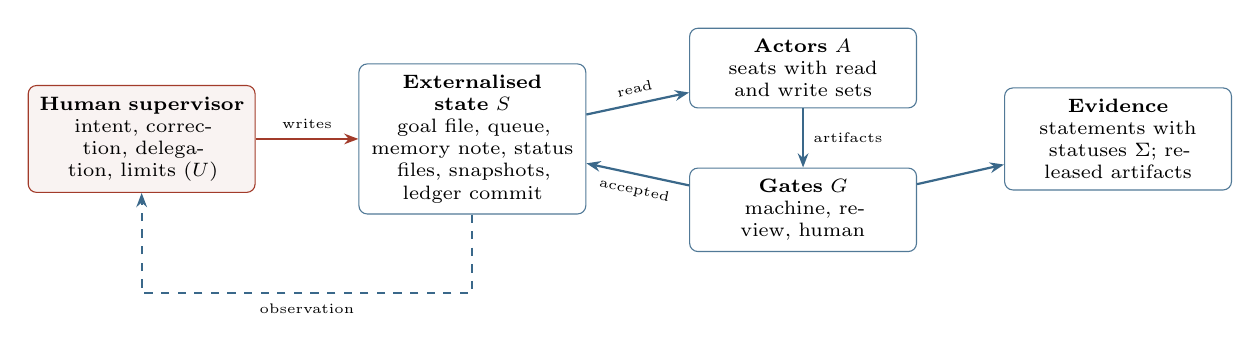
\begin{tikzpicture}[
  bx/.style={draw=linkblue!75,fill=white,rounded corners=3pt,align=center,font=\scriptsize,inner sep=4pt,minimum height=1cm,text width=2.6cm},
  hb/.style={bx,draw=humanred,fill=humanred!6},
  arr/.style={-{Stealth[length=1.8mm]},thick,draw=linkblue!85}]
\node[hb] (h) at (0,0) {\textbf{Human supervisor}\\ intent, correction, delegation, limits ($U$)};
\node[bx] (s) at (4.2,0) {\textbf{Externalised state $S$}\\ goal file, queue, memory note, status files, snapshots, ledger commit};
\node[bx] (a) at (8.4,0.9) {\textbf{Actors $A$}\\ seats with read and write sets};
\node[bx] (g) at (8.4,-0.9) {\textbf{Gates $G$}\\ machine, review, human};
\node[bx] (o) at (12.4,0) {\textbf{Evidence}\\ statements with statuses $\Sigma$; released artifacts};
\draw[arr,draw=humanred] (h) -- node[font=\tiny,above]{writes} (s);
\draw[arr] (s) -- node[font=\tiny,above,sloped]{read} (a);
\draw[arr] (a) -- node[font=\tiny,right]{artifacts} (g);
\draw[arr] (g) -- node[font=\tiny,below,sloped]{accepted} (s);
\draw[arr] (g) -- (o);
\draw[arr,dashed] (s.south) -- ++(0,-1.0) -| node[font=\tiny,pos=0.25,below]{observation} (h.south);
\end{tikzpicture}
\caption{The research loop as a supervised control system. The human acts
only through the control channel, whose inputs are written into the
externalised state; actors read the state and propose artifacts; gates decide
which artifacts and statuses enter the state and which are released.}
\label{fig:model}
\end{figure}

The remainder of the paper instantiates the model.
Section~\ref{sec:intents} describes how intents become goal files and how the
state survives across ticks; Sections~\ref{sec:reasoning}
and~\ref{sec:ledger} describe the actors and gates of derivation and
formalization; Section~\ref{sec:plane} describes how actors are given
machines and identity routes; Sections~\ref{sec:publication}--\ref{sec:outreach}
describe release; and Section~\ref{sec:steering} analyses the control channel
on the case study. Box~\ref{box:terms} and Table~\ref{tab:legend} fix the
vocabulary.

\begin{protocol}{Terms and labels}
\label{box:terms}
\begin{description}[leftmargin=0pt,itemsep=1pt,font=\normalfont\bfseries]
\item[Intent] A short natural-language directive that fixes an objective,
constraints and delegation, with its provenance: who, when, what counts as
success. The team informally calls it a \emph{wish}.
\item[Line] One research effort that follows from an intent, with its own goal
file, queue and objects; a \emph{lane} is the line's suffix in branch and
worktree names.
\item[Owner] The human principal of a line, who states its intents and holds
the standing decisions; in this paper, one of the authors.
\item[Orchestrator] The coordinating agent session that runs a line.
\item[Goal file] The persistent, machine-readable form of an intent, which
every agent of the line reads before acting.
\item[Queue] The line's log of rounds: what was derived, sent, pending.
\item[Memory note] The owner's instructions in their own words, the objects
the line owns, and its cleanup scope.
\item[Status file] A file each remote agent overwrites after every material
step: unit, phase, next step.
\item[Tick] One wake-up of the orchestrator's self-paced loop.
\item[Seat] A role filled by one agent with its own context: orchestrator,
author, referee, delegated job, build-machine agent, managed agent, review
loop.
\item[Round] One cycle of derivation, checking and drafting on a paper.
\item[Numbered snapshot] A frozen copy of the drafts that referees read.
\item[Unit] One preregistered piece of formalization, taken to merge or to
a named obstacle.
\item[Ledger] The trureturing library of kernel-checked Lean modules.
\item[Frozen] A ledger module accepted by the kernel and recorded with its
statement identity.
\item[Escape witness] A new intermediate proposition on a proof's live path
that binding existing results cannot produce.
\item[Bind-only] A declaration that only instantiates, substitutes,
projects, recombines or normalizes existing results.
\item[Route] A named path from an agent to a service through the
credential broker.
\item[Task log] The outreach coordinator's durable record of tasks and their
states.
\end{description}
\end{protocol}

\begin{table}[htbp]
\centering\footnotesize
\caption{One legend for the four status vocabularies of the system.}
\label{tab:legend}
\begin{tabularx}{\linewidth}{@{}>{\raggedright\arraybackslash}p{0.2\linewidth}>{\raggedright\arraybackslash}p{0.22\linewidth}>{\raggedright\arraybackslash}p{0.22\linewidth}>{\raggedright\arraybackslash}X@{}}
\toprule
Statement status (drafts) & Book badge & Mathesis rubric & Meaning \\
\midrule
\textsc{lean} & green Lean badge & verified with Lean & Every cited declaration is a frozen theorem of the ledger \\
\textsc{proved} & violet written proof & correctness \status{correct} & Complete proof in the text, not yet formalized \\
\textsc{classical} & remark, ``literature result'' & literature \status{supported} & Exact reference to the literature \\
\textsc{hypothesis} & remark & --- & A named physical or structural input \\
\textsc{conjecture} & red open badge & conjecture record & Stated with evidence, unproved \\
\textsc{programme} & remark & --- & A direction, with what would have to be shown \\
\textsc{refuted} & remark with correction & correctness \status{error} & False as stated; counterexample and corrected statement kept \\
\bottomrule
\end{tabularx}
\par\smallskip\raggedright\footnotesize
Formal units carry their own phases in the status file:
\code{prereg}, \code{probe}, \code{implement}, \code{review}, \code{pr-open},
\code{merged}, \code{cleaned}, \code{blocked}. A remark from an unpublished
derivation is labelled ``manual derivation''.
\end{table}

\section{The research and dissemination loops}
\label{sec:loop}
The method runs as two coupled loops (Figure~\ref{fig:loop}). The
\emph{research loop} turns an intent into checked drafts and merged formal
units; its ticks come every twenty minutes or so and its rounds about once
an hour. The \emph{dissemination loop} takes each resolved result of the
ledger and, in parallel, writes it back to the books and produces a short
note, which goes both to Mathesis and into a letter to the problem's authors;
its coordinator runs four times an hour, and replies arrive whenever their
authors write. Replies and human corrections feed the next intents.

\begin{figure}[t]
\centering
\resizebox{\linewidth}{!}{%
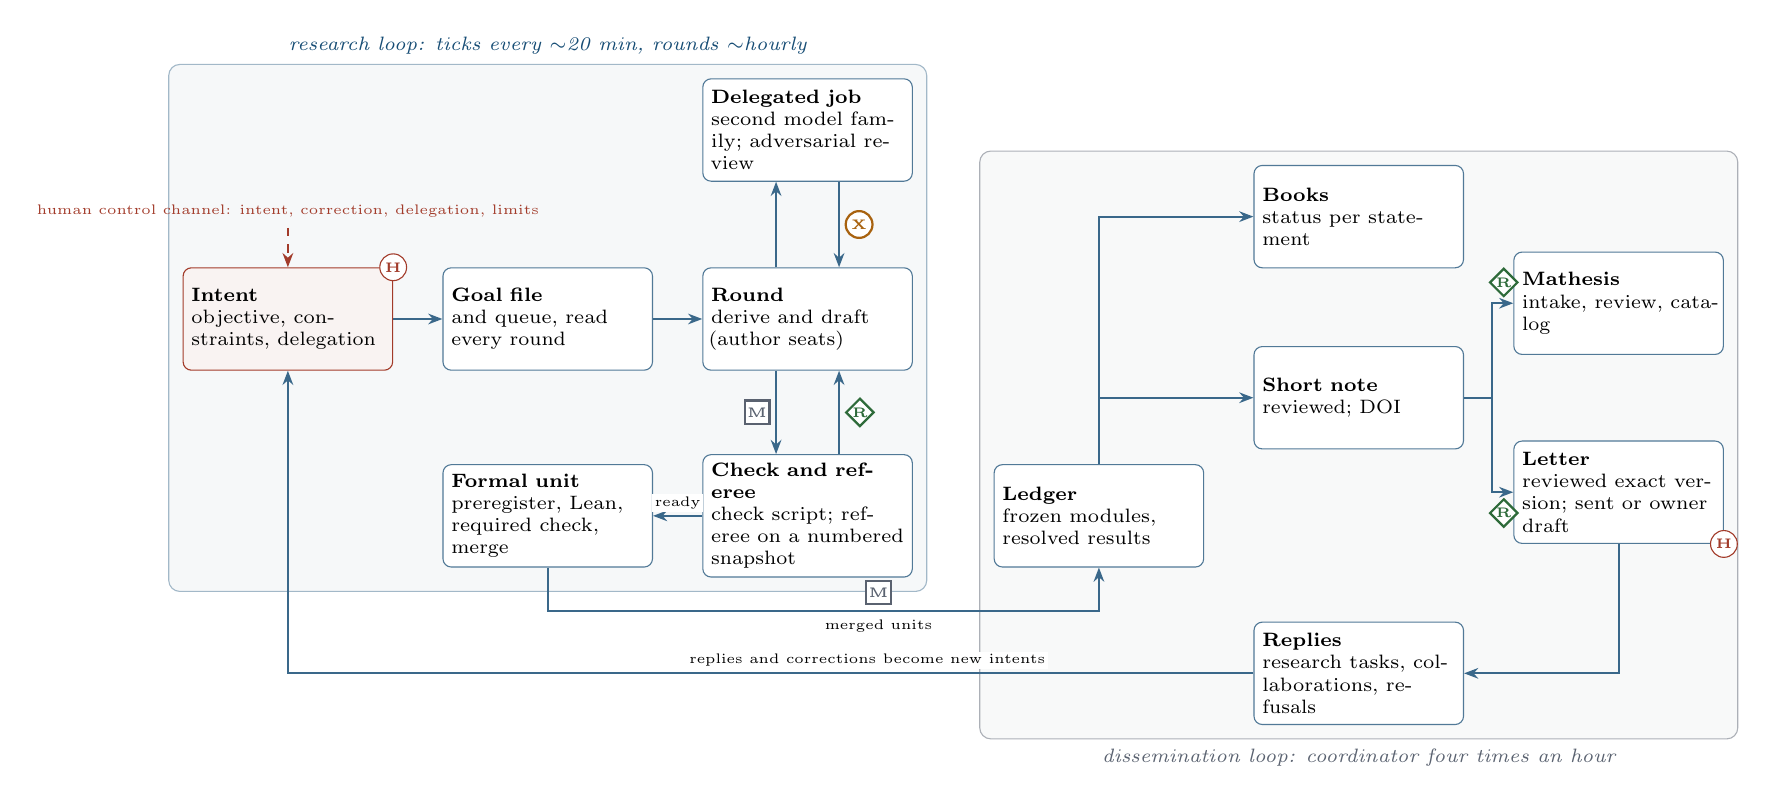
\begin{tikzpicture}[
  st/.style={draw=linkblue!75,fill=white,rounded corners=3pt,
    text width=2.45cm,minimum height=1.3cm,align=left,font=\scriptsize,inner sep=3pt},
  hu/.style={st,draw=humanred,fill=humanred!6},
  arr/.style={-{Stealth[length=1.8mm]},thick,draw=linkblue!85},
  lab/.style={font=\tiny,fill=white,inner sep=1pt,align=center},
  gm/.style={rectangle,draw=planegray,fill=white,text=planegray,font=\tiny\bfseries,inner sep=1pt,minimum size=3mm},
  gr/.style={diamond,draw=reviewgreen,fill=white,text=reviewgreen,font=\tiny\bfseries,inner sep=0.3pt,minimum size=3.6mm},
  gx/.style={circle,draw=standorange,fill=white,text=standorange,font=\tiny\bfseries,inner sep=0.5pt,minimum size=3.4mm},
  gh/.style={circle,draw=humanred,fill=white,text=humanred,font=\tiny\bfseries,inner sep=0.5pt,minimum size=3.4mm}]
\node[hu] (wish) at (0,0) {\textbf{Intent}\\ objective, constraints, delegation};
\node[st] (goal) at (3.3,0) {\textbf{Goal file}\\ and queue, read every round};
\node[st] (round) at (6.6,0) {\textbf{Round}\\ derive and draft (author seats)};
\node[st] (deleg) at (6.6,2.4) {\textbf{Delegated job}\\ second model family; adversarial review};
\node[st] (check) at (6.6,-2.5) {\textbf{Check and referee}\\ check script; referee on a numbered snapshot};
\node[st] (unit) at (3.3,-2.5) {\textbf{Formal unit}\\ preregister, Lean, required check, merge};
\draw[arr] (wish) -- (goal);
\draw[arr] (goal) -- (round);
\draw[arr] ([xshift=-4mm]round.north) -- ([xshift=-4mm]deleg.south);
\draw[arr] ([xshift=4mm]deleg.south) -- node[gx,right=2pt]{X} ([xshift=4mm]round.north);
\draw[arr] ([xshift=-4mm]round.south) -- node[gm,left=2pt]{M} ([xshift=-4mm]check.north);
\draw[arr] ([xshift=4mm]check.north) -- node[gr,right=2pt]{R} ([xshift=4mm]round.south);
\draw[arr] (check) -- node[lab,above=1pt]{ready} (unit);
\node[st] (ledger) at (10.3,-2.5) {\textbf{Ledger}\\ frozen modules, resolved results};
\node[st] (books) at (13.6,1.3) {\textbf{Books}\\ status per statement};
\node[st] (note) at (13.6,-1.0) {\textbf{Short note}\\ reviewed; DOI};
\node[st] (mathesis) at (16.9,0.2) {\textbf{Mathesis}\\ intake, review, catalog};
\node[st] (letter) at (16.9,-2.2) {\textbf{Letter}\\ reviewed exact version; sent or owner draft};
\node[st] (reply) at (13.6,-4.5) {\textbf{Replies}\\ research tasks, collaborations, refusals};
\draw[arr] (unit.south) -- ++(0,-0.55) -| node[gm,pos=0.3,above=2pt]{M} node[lab,pos=0.3,below=2pt]{merged units} (ledger.south);
\draw[arr] (ledger.north) |- (books.west);
\draw[arr] (ledger.north) |- (note.west);
\draw[arr] (note.east) -- ++(0.35,0) |- node[gr,pos=0.78,above=2pt]{R} (mathesis.west);
\draw[arr] (note.east) -- ++(0.35,0) |- node[gr,pos=0.78,below=2pt]{R} (letter.west);
\draw[arr] (letter.south) |- (reply.east);
\draw[arr] (reply.west) -| node[lab,pos=0.2,above=1pt]{replies and corrections become new intents} (wish.south);
\draw[arr,dashed,draw=humanred] ([yshift=5mm]wish.north) node[above,font=\tiny,text=humanred]{human control channel: intent, correction, delegation, limits} -- (wish.north);
\node[gh] at (wish.north east) {H};
\node[gh] at (letter.south east) {H};
\begin{scope}[on background layer]
\node[draw=linkblue!40,fill=linkblue!4,rounded corners=4pt,inner sep=5pt,fit=(wish)(goal)(round)(deleg)(check)(unit),
  label={[font=\scriptsize\itshape,text=linkblue,anchor=south]north:research loop: ticks every $\sim$20 min, rounds $\sim$hourly}] {};
\node[draw=planegray!50,fill=planegray!4,rounded corners=4pt,inner sep=5pt,fit=(ledger)(books)(note)(mathesis)(letter)(reply),
  label={[font=\scriptsize\itshape,text=planegray,anchor=north]south:dissemination loop: coordinator four times an hour}] {};
\end{scope}
\end{tikzpicture}}
\caption{Two coupled loops. In the research loop an intent becomes a goal file;
rounds derive and draft; a check script (\textcolor{planegray}{\textbf{M}},
machine gate) and a referee on a numbered snapshot
(\textcolor{reviewgreen}{\textbf{R}}, review gate) close each round;
delegated work returns through cross-family review
(\textcolor{standorange}{\textbf{X}}); ready statements become formal units
admitted by the kernel and the required check (\textbf{M}). In the
dissemination loop each resolved result is written back to the books and
becomes a short note; the reviewed note goes to Mathesis and into a letter in
parallel (\textbf{R}). \textcolor{humanred}{\textbf{H}} marks where people
act: intents and corrections, and letters routed to the owner. Replies and
corrections feed new intents. All steps run on the execution and identity
plane of Section~\ref{sec:plane}.}
\label{fig:loop}
\end{figure}

\begin{table}[htbp]
\centering\scriptsize
\caption{Components: input, output, gate (M machine, R review, X cross-family,
H human), cadence and the artifact that persists.}
\label{tab:overview}
\begin{tabularx}{\linewidth}{@{}>{\raggedright\arraybackslash}p{0.1\linewidth}>{\raggedright\arraybackslash}p{0.13\linewidth}>{\raggedright\arraybackslash}p{0.15\linewidth}>{\raggedright\arraybackslash}X>{\raggedright\arraybackslash}p{0.13\linewidth}>{\raggedright\arraybackslash}p{0.15\linewidth}@{}}
\toprule
Component & Input & Output & Gate & Cadence & Persisted artifact \\
\midrule
Intent, goal file & A directive & Goal file, queue entry & H; rules file outranks goal file & On demand & Goal file, memory note \\
Reasoning loop & Goal file, reports & Drafts, delegated results & M check script; R referee; X adversarial review & Ticks $\sim$20 min; rounds $\sim$hourly & Drafts, check scripts, numbered snapshots, reports \\
Ledger & Preregistered unit & Frozen modules, result markers & M kernel, axioms, frozen state, typed refutation, required check; R proof shape, admission basis & Preregistration to merge 1--4 h & Issue, pull request, frozen state file \\
Books, notes & Frozen modules, settled results & Editions, notes with DOI & M book checks; R note review & Book PRs merged within 45 min & Book commit, Zenodo record \\
Mathesis & Papers, notes, conjectures & Accepted records, Lean targets & R four stages; policy function & Catalog hourly & Record, catalog entry \\
Outreach & Resolved results, replies & Letters, owner drafts, tasks & R exact-version review; M refusal and mailbox checks; H owner letters & Coordinator 4$\times$/hour & Task log, verdict, sent copy \\
Plane & Agents, machines & Sandboxes, worktrees, routes & Brokered credentials; owner approval of new routes & Continuous & Grants, sessions \\
\bottomrule
\end{tabularx}
\end{table}

\paragraph{The life of one intent.} The owner asked whether the AXIOM-$\Omega$
axioms made sense and, after a first draft, wrote: open a goal and keep
going. The orchestrator wrote a goal file and started its loop. Each round it
derived new statements, ran a check script, and sent them to two author seats;
referees read numbered snapshots. A statement ready for the library became
unit~1: preregistered as a public issue, proved in Lean on the build machine,
merged 3~h~46~min after its preregistration. Stabilized results went back to
the book in small pull requests. The owner's next sentences---three papers, write
back to the book, delegate hard problems, absorb the rest of the book---each
changed the loop within one tick.

\subsection{Cast and deployment}
\label{sec:cast}
Table~\ref{tab:cast} and Figure~\ref{fig:cast} name every seat with its model
or tool, the machine it runs on, its identity route and what it may write.
The \emph{first model family} is Anthropic's Claude: the orchestrator runs as
a Claude Code session on Claude Fable~5.2, and its author and referee
subagents run on Claude Opus~5.5. The \emph{second model family} is
OpenAI's: Codex runs the delegated command-line jobs, the build-machine
agents and the managed agents, and GPT Pro, reached as a chat product through
the broker, serves as an oracle for route-finding and figures.

\begin{table}[htbp]
\centering\scriptsize
\caption{Cast and deployment: who runs where, under which route, and what each
seat may write.}
\label{tab:cast}
\begin{tabularx}{\linewidth}{@{}>{\raggedright\arraybackslash}p{0.15\linewidth}>{\raggedright\arraybackslash}p{0.17\linewidth}>{\raggedright\arraybackslash}p{0.15\linewidth}>{\raggedright\arraybackslash}p{0.19\linewidth}>{\raggedright\arraybackslash}X@{}}
\toprule
Seat & Model or tool & Machine & Identity route & May write \\
\midrule
Orchestrator & Claude Code, Claude Fable 5.2 & A local workstation & The owner's session; broker routes for remote work & Goal files, queue, memory note, book pull requests \\
Author seats & Claude Opus 5.5 subagents & Same & The session & Their own paper's draft and check scripts \\
Referee seats & Claude Opus 5.5 subagents, fresh context & Same & The session & Their own report folder only \\
Delegated jobs & Codex command line, extra-high effort & Same & Local command-line client & Their own task directory only \\
Oracle & GPT Pro chat product & Hosted & Broker route by service name & Nothing; answers only \\
Build-machine agents & Codex under heca & Shared build machine & Reached through the broker's SSH execution; code-hosting access on the machine & Own worktrees, scratch directory, status file, library pull requests \\
Managed agents & Codex on CMA & CMA sandboxes & Scoped broker credentials & Own drafts and research artifacts; no mail, no verdicts \\
Review loop & Claude, person-started & A local workstation & The session; HMAC review key & Verdicts, contact tables, staging \\
Outreach coordinator & Program on hosted CI & Hosted runner & Dedicated broker session & Task log; sends after a verdict \\
Mathesis referee and auditor & GPT Pro; Codex on CMA & Mathesis service & Broker routes & Stage reports \\
\bottomrule
\end{tabularx}
\end{table}

\begin{figure}[htbp]
\centering
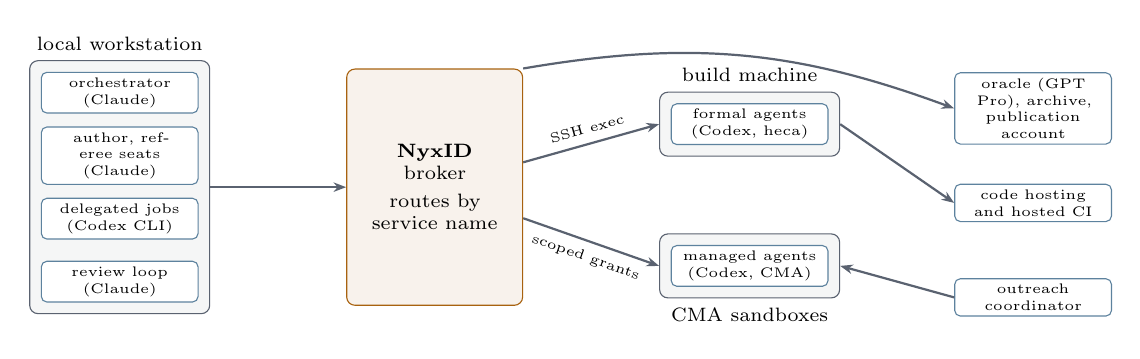
\begin{tikzpicture}[
  mach/.style={draw=planegray,fill=planegray!6,rounded corners=3pt,inner sep=4pt,align=center,font=\scriptsize},
  seat/.style={draw=linkblue!70,fill=white,rounded corners=2pt,font=\tiny,align=center,inner sep=2pt,text width=1.85cm},
  arr/.style={-{Stealth[length=1.6mm]},thick,draw=planegray}]
\node[seat] (orch) at (0,0) {orchestrator\\(Claude)};
\node[seat] (auth) at (0,-0.8) {author, referee seats\\(Claude)};
\node[seat] (cli) at (0,-1.6) {delegated jobs\\(Codex CLI)};
\node[seat] (rl) at (0,-2.4) {review loop\\(Claude)};
\begin{scope}[on background layer]\node[mach,fit=(orch)(auth)(cli)(rl),label={[font=\scriptsize]above:local workstation}] (pc) {};\end{scope}
\node[draw=standorange,fill=standorange!8,rounded corners=3pt,font=\scriptsize,align=center,minimum height=3cm,text width=2cm] (nyx) at (4,-1.2) {\textbf{NyxID}\\ broker\\[2pt] routes by\\ service name};
\node[seat] (hecaag) at (8,-0.4) {formal agents\\(Codex, heca)};
\begin{scope}[on background layer]\node[mach,fit=(hecaag),label={[font=\scriptsize]above:build machine}] (bm) {};\end{scope}
\node[seat] (cmaag) at (8,-2.2) {managed agents\\(Codex, CMA)};
\begin{scope}[on background layer]\node[mach,fit=(cmaag),label={[font=\scriptsize]below:CMA sandboxes}] (cm) {};\end{scope}
\node[seat] (svc) at (11.6,-0.2) {oracle (GPT Pro), archive, publication account};
\node[seat] (gh) at (11.6,-1.4) {code hosting and hosted CI};
\node[seat] (coord) at (11.6,-2.6) {outreach coordinator};
\draw[arr] (pc.east) -- (nyx.west);
\draw[arr] (nyx) -- node[font=\tiny,above,sloped]{SSH exec} (bm.west);
\draw[arr] (nyx) -- node[font=\tiny,below,sloped]{scoped grants} (cm.west);
\draw[arr] (nyx.north east) to[bend left=15] (svc.west);
\draw[arr] (bm.east) -- (gh.west);
\draw[arr] (coord.west) -- (cm.east);
\end{tikzpicture}
\caption{Deployment. Seats on a local workstation reach remote machines and
services only through broker routes; build-machine and managed agents receive
scoped access; gates run on hosted continuous integration.}
\label{fig:cast}
\end{figure}

\section{Intent specification and the goal file}
\label{sec:intents}
\paragraph{What an intent looks like.} An intent is one or two sentences. The
AXIOM-$\Omega$ line began with the question whether the axioms of one book
chapter make sense in the light of the current library, and grew with
``write me a draft first; unify as far as possible; fill the gaps''. An intent
names a goal, sometimes a scope or a deliverable, and rarely a method; the
system supplies the method.

\paragraph{From intent to goal file.} When an intent needs more than one round,
the orchestrator writes a goal file, the persistent, machine-readable form of the intent
that every agent of the line reads before acting. Box~\ref{box:goal} gives
the anatomy of the goal file that briefed the formalization agent of the
AXIOM-$\Omega$ line.

\begin{protocol}{Anatomy of a goal file (AXIOM-$\Omega$ formalization line)}
\label{box:goal}
\begin{enumerate}[leftmargin=*,itemsep=1pt]
\item \textbf{Objective.} One line: formalize the round-trip comparison
closure of AXIOM-$\Omega$ in the library and write the results back.
\item \textbf{Authority and house rules.} The repository's rules file and its
skills govern; where the goal file disagrees, the rules win and the
disagreement is recorded. Preregister before any Lean probe. Work only in a
linked worktree. Delivery means push, pull request, required checks green,
merged, and the first push to the development branch verified; the line
merges its own pull requests.
\item \textbf{Bounds on shared resources.} Touch only objects the line
created; stop only processes it started, by recorded identifier; keep Lean
builds targeted and use at most six build threads while the machine is
loaded.
\item \textbf{Identity and files.} The orchestrating session and its resume
command; a suffix used in every lane, branch and worktree name; one scratch
directory for all non-repository files; the source draft and its numerical
check scripts.
\item \textbf{Mathematical content.} Definitions and hypotheses, the claims
to be proved with a proof route for each, the literature already read (to be
cited, not formalized), and the proposed non-binding facts that will carry
new content.
\item \textbf{Units.} The first unit fully specified; later units listed,
each to be preregistered separately after the previous one is delivered or
blocked.
\item \textbf{Stopping rule.} One round is one unit taken to merge or to a
named obstacle; a unit that does not close is reported with its obstacle,
and that report is a result.
\item \textbf{Cleanup scope.} After each delivered unit, return the worktree
and delete the files the line created outside the repository; report disk
usage before and after.
\item \textbf{Status file.} After every material step the agent overwrites a
status file with: time, session, unit, phase (\code{prereg}, \code{probe},
\code{implement}, \code{review}, \code{pr-open}, \code{merged},
\code{cleaned}, \code{blocked}), issue, pull request, worktree, branch,
running build processes, frozen identifiers, obstacle and next step.
\end{enumerate}
\end{protocol}

A second goal file continued the line after the first unit: it named five
further units in order, the proposed new content of each, the literature
state, and a cost rule (the provider's default model at high rather than
maximal effort, targeted builds).

\paragraph{How the loop paces itself.} The orchestrator runs as a
self-paced loop. Each tick follows a fixed prompt: read the remote agent's
status file; if the agent is idle or blocked, read its log and send the
mathematical answer or the next unit's instruction; confirm merges and
verify the first push to the development branch; continue the open
derivations in the drafts and recompile them; clean up after each delivered
unit; and stop the loop when all units are delivered and the drafts agree
with the formalization. Between ticks the orchestrator schedules its own
wake-ups and attaches monitors to long jobs---a build, a check run, a
delegated job---so that it resumes when they finish. Over the two days of the
AXIOM-$\Omega$ line the loop ran about twenty ticks and scheduled several
dozen wake-ups.

\paragraph{How a correction propagates.} A correction is written into the
memory note in the owner's words with its date, summarized as a dated entry
in the queue, and quoted in the tick prompt that the loop runs from then on.
When the owner wrote \zh{别这么多 之后系统内存不够卡死了} (``not so many---the
system will run out of memory and freeze''), the next queue entry recorded
that fourteen delegated jobs had been stopped by their recorded process
identifiers and marked as queued, that at most about four would run at once,
and the order of the rest; the following tick prompt carried the cap and the
memory check. Formats are given in Appendix~\ref{app:templates}.

\paragraph{How state survives.} A line runs for days and outlives the
context of any single agent. Three files carry its state. The \emph{queue}
logs each round with the time at which its state was read, what was sent,
what is ready to send, and what is still to be derived. The \emph{memory
note} records the owner's instructions in their own words, the objects the
line owns, and its cleanup scope. The remote agent's \emph{status file}
carries the formal unit's phase. When the orchestrator's context is
compacted, the next tick begins by reading the memory note and the queue and
re-measuring what they describe; the AXIOM-$\Omega$ line passed through two
such compactions without losing a unit.

\section{Gated multi-agent derivation}
\label{sec:reasoning}
\paragraph{Statuses.} Every statement carries one status:
\textsc{proved} (complete proof in the text), \textsc{lean} (a library
declaration, cited by file and name), \textsc{classical} (an exact reference),
\textsc{hypothesis} (a named physical or structural input),
\textsc{conjecture} (stated with evidence), \textsc{programme} (a direction,
with what would have to be shown) or \textsc{refuted} (a claim that is false
as stated, with the counterexample and the corrected statement). Refutations
are kept as results: a refuted claim tells the next reader which route is
closed and why, and the corrected statement often becomes the next
theorem. Table~\ref{tab:legend} maps them onto the book badges and the Mathesis rubric.

\paragraph{Seats.} Each round uses three kinds of seat. The
\emph{orchestrator} derives new statements, writes the numerical checks and
decides what goes into the next round. \emph{Author seats} (Claude subagents,
one per paper) write the derivations into the paper, verify them,
and repair what referees find. \emph{Referee seats} are fresh subagents that
read a numbered snapshot of the drafts and report errors, gaps, novelty
problems and overstatements. A referee is told to write only in its own
report folder, to read the authors' own gap list last so that it does not
anchor the judgement, to check every theorem line by line, and to test each
claim on examples and near-counterexamples of its own; its report lists
findings as blocking or minor, each with the statement it concerns, and the
next round answers each finding. A later referee may be asked to check that
earlier findings were addressed. The prompt is in Appendix~\ref{app:templates}. The oracle, GPT Pro reached through the
broker, proposes literature maps, proof routes and figures; an executing seat
verifies what it proposes.

\paragraph{Delegation to a second model family.} A problem that the
orchestrator cannot close in a round is written up as a task and handed to a
Codex command-line job of the second model family; its adversarial review is
another such job, and verification is done by the first family's author
seat and referee. Box~\ref{box:delegate} gives the protocol; the task files are in
Appendix~\ref{app:templates}.

\begin{protocol}{Delegating a hard problem}
\label{box:delegate}
\begin{enumerate}[leftmargin=*,itemsep=1pt]
\item \textbf{Task file.} The problem statement, the exact pages and labels
of the paper to read (read-only), what to produce, and the standard: complete
proofs, exact citations, nothing called a theorem without one of them.
\item \textbf{Deliverables.} A self-contained section, a bibliography, a
check script that tests every identity, inequality and example and must pass,
and a status table assigning each statement one of the labels below, with a
list of differences from the source and ``what a referee should attack
first''.
\item \textbf{Adversarial review.} A second job, in a fresh context, acts as
a hostile referee: for every inference it decides correct, gap (with repair)
or wrong (with counterexample), and it checks the hypotheses of every cited
theorem.
\item \textbf{Verification and integration.} The paper's author-agent
verifies the repaired proof and writes it into the paper; a referee seat
then reviews the new section.
\item \textbf{Resources.} At most about four jobs run at once; each is
started with its process identifier recorded, and memory pressure and swap
are read before each start.
\end{enumerate}
\end{protocol}

In the AXIOM-$\Omega$ line a delegated job proved a roundness theorem for the
mathematical paper; the adversarial review found two small gaps, which were
repaired; the author-agent verified and integrated the proof; and a referee
seat confirmed it ``correct as stated''. Another job answered a one-sided
variant of the question negatively with a counterexample, which passed its
adversarial review and was re-derived by a cross-paper referee.

\paragraph{Numerical checks as a gate.} Each round has a check script that
tests every identity, inequality and example the round introduces, and the
round's new statements are sent together with a passing script. In the
AXIOM-$\Omega$ line the scripts ran from a few dozen to over nine thousand
checks per round. A check is labelled as numerical evidence for the
statement it tests.

\paragraph{Numbered snapshots.} Before a referee round the orchestrator copies
the drafts into a numbered snapshot; referees read the snapshot, and the
author seats keep editing the live drafts. Each finding can therefore be
traced to the exact text it concerns. As of 07:57~UTC on 20 November 2026 the
mathematical draft was at round~23 and the physical draft at round~24; the
line had kept sixteen numbered snapshots, with five referee rounds on each
paper and two reading both.

\subsection{Records retained at handoffs}
\label{sec:records}
The method requires each handoff to retain the mathematical statement version
and the evidence associated with it. A result record links assumptions and
conclusion to a readable argument, supporting artifacts and contributors,
following established provenance concepts \citep{prov}; for mathematics it
must also identify which statement an activity establishes
(Table~\ref{tab:records}). When assumptions or conclusion change, the method
creates a new statement version and keeps the earlier one; a check of one
version does not certify a strengthened version.

\begin{table}[htbp]
\centering\small
\caption{Information the method requires each handoff to retain, and the
artifact that carries it. Evidence is attached to the version it supports.}
\label{tab:records}
\begin{tabularx}{\linewidth}{@{}>{\raggedright\arraybackslash}p{0.17\linewidth}>{\raggedright\arraybackslash}X>{\raggedright\arraybackslash}p{0.3\linewidth}@{}}
\toprule
Object & Retained information & Carried by \\
\midrule
Intent & Who stated it, when, the exact question or artifact, any success criterion & Memory note and queue \\
Result version & Assumptions, conclusion, readable proof or computation, roles & Draft at a numbered snapshot \\
Check & Target statement, evidence type, environment, outcome, scope & Check script and its output \\
Feedback response & Criticism, affected statement, research action, checked outcome & Referee report and the next round's gap list \\
Public artifact & Version, identifier, ledger commit, status per statement & Book commit, Zenodo record, Mathesis record \\
Knowledge relation & Used result version, nature of the dependency, evidence & Lean imports; citations in the draft \\
Proof contribution & Contributor, formal statement, source, independent check & Preregistration issue and pull request \\
\bottomrule
\end{tabularx}
\end{table}

\section{The formally verified ledger}
\label{sec:ledger}
trureturing \citep{trureturingrepo} is a public repository with three parts:
theory volumes that serve as input, the Lean source that is the only carrier
of mathematical truth, and a harness that validates, emits documents and
guards admission. Mathlib is a pinned dependency \citep{mathlib}. As of 20
November 2026 the library holds 16{,}436 Lean source files, 14{,}832 frozen
modules and 4{,}511 files of escape registrations; more than 21{,}000 pull
requests have been merged, and six workflows and five repository skills
serve contributors.

\paragraph{The rules file.} One rules file, read by every human and agent
contributor before acting, states what the repository asks: kernel-checked
truth, with everything else marked as input or bookkeeping; a status on every
statement, with \code{open} for what cannot be decided; preregistration
before probing; library before proof; no content-free declarations; one
linked worktree per task; disclosure of the skill, the seats and their model
families in every pull request and issue; and termination of processes only
by recorded identifier. Rules carry the date and words of the owner's ruling
that introduced them, so a contributor can see why a rule exists. The rules
file is written in Chinese; Appendix~\ref{app:templates} gives an English
summary. Five public skills turn the rules into procedures:
\code{formal-thinking-and-answer} (the default for every request),
\code{codex-formalize}, \code{autonomous-research}, \code{lean-optimize}
and \code{lean-fork-contribute}, all under \code{skills/} in the
repository.

\paragraph{Admission rules.}
\emph{Library before proof}: before writing Lean, an agent searches the
repository, the pinned Mathlib and admissible third-party libraries, and
imports an exact hit instead of re-proving it. \emph{No bind-only
declarations}: a declaration whose conclusion follows from existing results
by instantiation, substitution, projection, recombination and normalization
alone may not be added; a helper with a real consumer on a live proof path is
allowed, and so is the public conclusion of an open-problem settlement.
\emph{Two admission bases}: a first freeze needs either an escape witness---a
new intermediate proposition on the live proof path that the binding
operations cannot produce---or the verbatim settlement of a published, named
open problem that a literature check found unresolved.
\emph{Preregistration}: the expected new content is named in a public issue
before the probe, and a different observed witness requires a new
preregistration; reviewers check this convention. \emph{Computational
content}: bounded enumerations and certified instances enter only as verified
refutations of a named claim, typed as \code{Not claim}; a checker arrives
with a first concrete instance. \emph{Escape registration}: each new public
theorem is registered against a readout template in a separate package, and
the registration verdicts are warnings.

\paragraph{What decides admission.} The kernel, the axiom whitelist, the
frozen-state check, the typed-refutation check and the required continuous
integration are machine gates. The admission basis, the proof shape and the
faithfulness of a formal statement to its source are judged by model review,
with the seats and their model families disclosed in the pull request.

\paragraph{Frozen modules.} A module accepted by the kernel is frozen through
the canonical writer: a state file records its statement identity and ordered
declaration list, and a check compares membership with the current tree on
every change. Later work may re-pin a frozen module, for example when a
private lemma becomes public. Retracting a node requires retracting its
descendants, so a correction costs in proportion to the dependent subgraph.

\paragraph{Continuous integration.} One workflow detects the changed paths,
selects test units from an allowlist and exposes a single required check that
is green only if every selected unit ran and passed. Candidate code is
executed; the protected base is read only as data. Maintainers, agents and
forks pass the same gates. Strict up-to-date merging is off by an owner
ruling based on the measured catch-up cost, and checks on every push to the
development branch cover the remaining gap.

\begin{protocol}{The life of one formal unit}
\label{box:unit}
\begin{enumerate}[leftmargin=*,itemsep=1pt]
\item \textbf{Preregister.} Open a public issue that names the target
statement, the proposed non-binding facts and the admission basis, with the
creating session recorded.
\item \textbf{Search.} Search the library, Mathlib and admissible libraries;
reuse exact hits and re-preregister if the new content shrinks.
\item \textbf{Worktree.} Create or reuse a linked worktree named with the
line's suffix; checkpoint after every recoverable step.
\item \textbf{Module.} Write the Lean module, its Blueprint entry and, for new
public theorems, the escape registration; decide and record the proof shape
of every declaration.
\item \textbf{Local build.} Build the target modules only, with bounded
threads; no \code{sorry}, no private axiom.
\item \textbf{Freeze.} Deposit the module through the canonical writer, which
writes its frozen state.
\item \textbf{Pull request.} Open it with \code{make pr}, which arms
auto-merge, and a provenance header (sessions, skills, seats and their model
families); the body records the proof shape and admission basis of every
declaration.
\item \textbf{Required check.} Wait with a single blocking command. If the
check fails because the build cache for the commit is missing, wait for the
cache-producing run of that commit, then rerun once; a second failure is
reported as the unit's obstacle.
\item \textbf{Merge and verify.} After the merge, verify the first push to
the development branch, close the preregistration issue, and record the
frozen identifiers in the status file.
\item \textbf{Clean up.} Return the worktree and delete the line's temporary
files; the next unit starts from the updated library.
\end{enumerate}
\end{protocol}

\paragraph{Remote formalization agents.} Formal units run on a shared build
machine, under heca, as Codex agents briefed by a goal file
(Box~\ref{box:goal}). The orchestrator addresses them through NyxID SSH: it
reads their status files and logs on each tick and sends the next instruction
or a mathematical answer as a message to the running agent. Each agent is
bounded by its goal file---its own worktree and scratch directory, a cap on
build threads, recorded process identifiers---and is replaced by a fresh
agent with a small context when its context grows large; a waiting agent uses
one blocking command for continuous integration instead of polling. In the
AXIOM-$\Omega$ line three units were merged in one day: a rank-one
classification from faithful round-trip comparison, the rigidity of the
continuous cosine doubling equation on the circle, and the reduction of a
two-readout law to d'Alembert's functional equation; a fourth unit was
preregistered and opened the next day \citep{prereg31739,axiomprs}.%
\footnote{The public issue titles number the units 1, 7, 8 and 9: the first
goal file reserved units 2--6 for later, and the second goal file continued
with unit~7.} From preregistration to merge the three units took 3~h~46~min,
1~h~09~min and 1~h~08~min; from pull request to merge, 2~h~13~min, 38~min and
39~min. Appendix~\ref{app:templates} shows the structure of a public
preregistration issue and of a pull-request header.

\section{The execution and identity plane}
\label{sec:plane}
Every step of the loop needs three things: an identity that a service will
trust, credentials for model providers, code hosting, mail and publication,
and a place to run with a working tree. A small team owns all of these
through a few people and a few machines. Three systems turn that small base
into a plane on which many agents work at once: NyxID routes identity and
credentials, heca runs long-lived agents on a build machine, and CMA runs
managed agents as a service. This section shows each system at work in the
AXIOM-$\Omega$ line and in the outreach and Mathesis pipelines, and then one
day of the loop seen plane by plane.

\subsection{NyxID: agents get capabilities, never secrets}
\label{sec:nyxid}
NyxID \citep{nyxid} is an open-source agent connectivity gateway. An agent
authenticates to NyxID and calls a service by name; NyxID injects the
credential into the proxied request, so the agent never sees a raw key or
OAuth token. Each agent or session holds a scoped token for the services its
task needs, and any session can be revoked without touching the underlying
credential. Credential nodes---node agents on private machines---reach
services behind NAT without a VPN or port forwarding. NyxID issues
short-lived SSH certificates and executes commands on remote hosts, provides
OpenID Connect sign-in with PKCE, service accounts and approval requests, and
wraps REST services as MCP tools. The team's oracle broker is registered in
NyxID as an ordinary service, and NyxID proxies requests to it.

\begin{protocol}{Setting up NyxID for a team (from its public documentation)}
\label{box:nyxid}
\begin{enumerate}[leftmargin=*,itemsep=1pt]
\item \textbf{Register a service.} \code{nyxid service add <service>} stores
the credential (an API key, an OAuth binding or an SSH configuration)
encrypted in NyxID, or on a credential node the team runs.
\item \textbf{Issue an agent key.} \code{nyxid api-key create --scopes
proxy}, then restrict the key to the services the agent needs with
\code{nyxid api-key update}.
\item \textbf{Point the agent at the proxy.} The agent calls
\code{/api/v1/proxy/...} or a provider endpoint such as
\code{/api/v1/llm/<provider>} by service name, or uses the MCP endpoint.
\item \textbf{Remote execution.} An SSH service in certificate or node-key
mode accepts \code{POST /api/v1/ssh/<service>/exec} with a command, a
principal from the service's allowed list and a timeout of 1--300 seconds;
the command-line form is \code{nyxid ssh exec}. Credential nodes
(\code{nyxid node}) reach machines behind NAT.
\item \textbf{Headless login.} Daemons such as heca sign in with the device
login protocol.
\item \textbf{Revoke.} Revoke an agent key or session; the stored
credential and the other routes are untouched.
\end{enumerate}
\end{protocol}

Table~\ref{tab:grants} shows which seat holds which route in the team's
loop; B marks a route brokered by NyxID, O a credential held outside the
broker.

\begin{table}[htbp]
\centering\scriptsize
\caption{Grant matrix: routes held by each seat (B brokered by NyxID; O held
outside the broker; blank: no route).}
\label{tab:grants}
\begin{tabular}{@{}lcccccc@{}}
\toprule
Seat & Code hosting & Oracle & CMA & Build-machine SSH & Mailbox & Publication \\
\midrule
Orchestrator session & O & B & & B & & \\
Build-machine agents & O (on the machine) & & & & & \\
Managed outreach agents & B & B & & & & \\
Outreach coordinator & B & B & B & & O & \\
Daily-report loop & & & & & & B \\
Mathesis service & & B & B & & & \\
\bottomrule
\end{tabular}
\end{table}

The mailbox is the one outreach route held outside the broker: the
coordinator keeps its own mailbox token, and only the coordinator sends.

\paragraph{At work in the loop.} The coordinating session of the AXIOM-$\Omega$
line never held a credential for the build machine. Every remote command went
through NyxID's SSH execution endpoint under a named principal:
\begin{center}\small
\code{nyxid ssh exec <build-machine-service> --principal <principal> -- '<command>'}
\end{center}
With this one route the session started remote agents, briefed them, sent
them messages, read their status files and logs, and cleaned up its own
scratch directory, while the broker held the key. The same broker fronts the
other services the system uses: the second model family's chat product, used
as an oracle for route-finding and figures, and the publication account that
posts the daily reports. Agents call these services by name, and a person can
revoke one route without touching the others. Inside the managed-agent
service, CMA asks NyxID for a missing service on an agent's behalf, and the
owner's approval delivers scoped credentials to the running sandbox
(Section~\ref{sec:cma}). Mathesis signs people in through NyxID and reaches
its referee and CMA through it; heca signs in to NyxID with a headless
device code.

\paragraph{The broker as a guardrail.} Because every remote command passes
through the broker, the broker can filter an agent's own traffic. On this
line one message to a remote agent was rejected because its text contained a
blocked pattern, a word for powering a machine off; the message was
reworded and sent again. The filter acts on what agents send, whatever their
intent, and the coordinating session treats a rejection as a signal to
rephrase.

\paragraph{A practical detail.} The SSH execution endpoint does not forward
standard input. Long briefs---a goal file, a source draft, a multi-page
instruction---were therefore shipped as base64 chunks in successive commands
and reassembled on the build machine before the agent read them. Another
team using a command-execution broker will meet the same constraint.

\paragraph{Design rule.} Agents get capabilities, never secrets; each seat
has its own route; every route can be cut independently.

\subsection{heca: long-lived agents on a build machine}
\label{sec:heca}
heca \citep{heca} is a daemon and command-line client that runs Claude and
Codex agents on a workstation; its binaries are published, its source is
not. An agent is created with a provider, a mode, a model, a
thinking level, a working directory or worktree and a first prompt;
workspaces, worktrees, sessions and teams are first-class; loops and
schedules run agents repeatedly; and permission policies answer or
pre-authorize permission requests. The team runs formal units on a shared
build machine under heca, where the Lean toolchain and build caches live and
an agent can spend hours on builds and continuous-integration waits. The
method uses a small subset of commands: \code{heca login} (device code
through NyxID); \code{heca agent create} with provider, mode, model, thinking
level, working directory or worktree path, and prompt; \code{heca agent
send}, \code{logs}, \code{status} and \code{usage}; \code{heca agent wait}
for an idle state with a timeout; and \code{loop} and \code{schedule}. Any
daemon that starts a command-line agent in a directory, accepts further
messages to it, and exposes its logs and status can stand in for heca.

\paragraph{At work in the loop.} Formalization on the AXIOM-$\Omega$ line ran
as long-lived agents on the build machine. Each was created with a provider,
a mode, a reasoning level, a working directory inside the formal library's
checkout, and a prompt that points at a goal file:
\begin{center}\small
\code{heca agent create --provider <provider> --mode <mode> --thinking <level> --cwd <library-checkout> --prompt '<read GOAL.md and begin>'}
\end{center}
The coordinating session then talked to the same agent with
\code{heca agent send}, read its usage with \code{heca agent status} and
\code{heca agent usage} (tokens in and out, message count), and read the
status file the agent maintains (unit, phase, next step) without waking it.
Three such agents ran on this line: the first carried the first unit to
merge; the second carried two units; a third, started fresh with a small
context, is carrying the next three.

\begin{protocol}{One formal unit, seen from the coordinating session}
\label{box:coord}
\begin{enumerate}[leftmargin=*,itemsep=1pt]
\item \textbf{Brief.} Ship the goal file and the source draft to the line's
scratch directory through the broker; create the agent, or send the next
unit to the running agent.
\item \textbf{Watch without waking.} On each tick read the status file
(unit, phase, issue, pull request, worktree, build processes, obstacle,
next step) and the agent's usage.
\item \textbf{Answer.} When the agent is idle or blocked, read its log and
send the mathematical answer or the decision it needs.
\item \textbf{Handle an infrastructure failure once.} If a check fails
because the build cache for the commit is missing, the agent waits for the
cache-producing run of that commit and reruns the check once; a second
failure is reported as the unit's obstacle.
\item \textbf{Verify.} After the merge, confirm the first push on the
development branch before the unit counts as done; then read the frozen
identifiers from the status file.
\item \textbf{Clean up.} The agent returns its worktree and deletes its
temporary files; the coordinating session deletes only objects it created
itself.
\item \textbf{Renew.} When the agent's context has grown large, start a
fresh agent for the next units with the same goal file.
\end{enumerate}
\end{protocol}

\paragraph{Rules learned on the line.} Five practices are now written into
every goal file. \emph{Single blocking waits}: an agent that polls
continuous integration with short waits re-reads its whole context on every
poll; one agent on this line reached a context of several hundred thousand
tokens and consumed tens of millions of input tokens, mostly from polling, so
agents wait with one blocking command and a new agent is started once the
context has grown. \emph{A status file per agent}, which the coordinator
reads without waking the agent. \emph{Ownership of objects}: the agent owns
its worktrees and cleans them; the coordinator touches only objects it
created. \emph{Wait for the cache-producing run of the commit, then rerun
once}: on one unit two reruns happened before this rule was fixed, and that
episode produced the rule.
\emph{Verify the first push} on the development branch before a unit is
called done.

\subsection{CMA: managed agents as a service}
\label{sec:cma}
CMA (ChronoAI Managed Agent) \citep{cma} is a cloud platform for running
coding agents. It manages their working environments, conversations,
approvals, service access and recovery; Codex is the supported agent
provider. Its runtime is nested: a \emph{sandbox} is an isolated runtime and
resource boundary; it holds \emph{workspaces}; each workspace holds
\emph{worktrees}; and each worktree holds exactly one \emph{agent}, whose
configuration and skills live in its own home. An agent is created from the
system image or an authorized image version, with inline model, reasoning,
permission, prompt and skill settings; live conversations run over the
public REST interface together with AG-UI or Responses, with the agent's
identifier as the thread. An agent starts with an empty workspace and
prepares its repository through the code-hosting API; that API grant does
not authenticate native Git transport, so agents read and write through the
API rather than with \code{git pull} and \code{git push}. When an agent
needs a service it lacks, a runtime capability asks for the owner's consent;
the request grants nothing until the owner approves, and the credentials then
arrive in the running sandbox without a restart. Conversations, turns and
recovery are durable. The coordinator sends each managed agent its pinned
inputs and prompt and receives its final message, its files and a structured
result.

\paragraph{What runs on CMA.} The outreach workflow runs every task kind as a
managed agent: short notes, first-contact research and drafting, replies,
research tasks, packages for Mathesis, and independent submissions. A
coordinator places them in a pool of sandboxes (at most four sandboxes with
six agents each, in two groups: notes, Mathesis packages and first contacts;
replies, research and submissions), with one model profile at high reasoning effort and two service
grants, code hosting and the oracle broker. In Mathesis every Codex step runs
on CMA: the audit of the referee's report against the source, advice, the
letter to the author, the plain-language explanation, Lean targets and Lean
probes.

\paragraph{How a managed job is specified.} Each task kind has a versioned
workflow definition. The first-contact definition, for example, fixes the
platform and provider; one durable task per item and version, with settings
pinned when the agent is created; the required inputs (the item and version,
the pinned commit of the library, the problem identifiers, the dossier with
the exact source, the result markers and Lean declarations, earlier receipts
and decisions, the contacts and thread ownership, the workflow and review
digest); the capabilities (read the pinned source and public literature,
read the contact policy, write its own draft and research artifacts); what is
forbidden (sending mail, posting, modifying upstream repositories, writing
review verdicts, spawning subworkers); the steps of Box~\ref{box:outreach};
seventeen hold codes; and the artifact contract: a versioned letter packet,
a research report bound to the item, version and workflow, and a digest of the
workflow and the review instructions. A missing capability is recorded as a
request for scoped provisioning, never worked around.

\paragraph{Binding a result to a verdict.} When a managed agent finishes, the
coordinator preserves its files in an immutable task record, reads them back,
and only then hands the exact result to the review loop. The verdict is
HMAC-authenticated and bound to the task revision, the hash of the result and
the hash of the workflow; a changed result or a changed workflow needs a new
review. A BOUNCE starts a new task carrying the previous result and the
feedback. The coordinator then stops the agent and retires a sandbox created
only for that task.

\paragraph{Why this matters for a small team.} The pipeline keeps its cadence
when no individual's machine is on: the coordinator runs four times an hour on
hosted continuous integration, and the managed agents run on the service.
Seats are separated by construction, since a drafting agent cannot send mail
or write a verdict. And every job leaves a record at the handoff: its inputs,
its files, the verdict and the receipt.

\subsection{Separation of seats, machines and credentials}
Seats are separated by process and context: the coordinating session, author
seats, referee seats, delegated jobs, build-machine agents and managed agents
are distinct agents with their own contexts. Machines are separated by role:
the coordinating session and the second-family command-line jobs run on a
local workstation; long Lean work runs on the shared build machine under
heca; outreach and Mathesis work runs in CMA sandboxes; gates run on hosted
continuous integration. Credentials are separated by brokering: no agent
holds a raw key, each holds a scoped token or a short-lived certificate, and
the owner of a service approves new grants. On shared machines a session
touches only objects it created and stops only processes it started, by
recorded identifier.

\begin{protocol}{Rebuilding the plane with other parts}
\label{box:rebuild}
\begin{description}[leftmargin=0pt,itemsep=1pt,font=\normalfont\bfseries]
\item[Essential] A secrets broker that injects credentials per route, revokes
per session and executes remote commands under a principal; a runner for
long-lived command-line agents on a machine with the proof toolchain and
caches, with send, logs and status; a sandbox service for short managed jobs
that cannot send mail or write verdicts; hosted continuous integration as the
only merge gate.
\item[Incidental] The particular products (NyxID, heca, CMA), the agent
providers, the chat interfaces, the image catalog and the trigger links. Any
broker, daemon and sandbox service with the essential properties will do.
\item[Order of setup] Broker first (services and agent keys), then the build
machine (toolchain, caches, daemon, remote execution), then the sandbox
service, then the coordinator on hosted CI.
\end{description}
\end{protocol}

\paragraph{Resource rule.} A small machine runs out of memory before it runs
out of ideas. Delegated jobs are therefore capped to a few at a time; each is
started with its process identifier recorded, so that it can be stopped on
its own; and the memory pressure and swap of the machine are read before each
start. When the owner found too many jobs running at once, the coordinating
session stopped the surplus by recorded identifier, marked them as queued,
and has since run them in a fixed order, about four at a time.

\subsection{One day of the loop, by plane}
\label{sec:oneday}
Table~\ref{tab:oneday} follows the AXIOM-$\Omega$ line through 20 November
2026, the day on which delegation, enlargement and the move of the drafts
into the book repository happened. Each row is a kind of activity recorded
in the line's queue.

\begin{table}[htbp]
\centering\footnotesize
\caption{One day of the loop (20 November 2026), by plane.}
\label{tab:oneday}
\begin{tabularx}{\linewidth}{@{}>{\raggedright\arraybackslash}p{0.17\linewidth}>{\raggedright\arraybackslash}p{0.17\linewidth}>{\raggedright\arraybackslash}p{0.16\linewidth}>{\raggedright\arraybackslash}X>{\raggedright\arraybackslash}p{0.13\linewidth}@{}}
\toprule
Activity & Where it ran & Identity route & Gate & Who decided \\
\midrule
Derivation rounds; the drafts reached rounds 23 and 24 by 07:57 UTC & Coordinating session and author subagents on a local workstation & The owner's session & Check script per round; referee findings addressed & Coordinating session within the goal \\
Delegated and adversarial jobs (a roundness proof and its review; a counterexample and its review; field and dimension audits; expansion modules, about four at a time) & Second-family command-line jobs on the same computer & Local command-line client & Check script passes; hostile review; author-agent verification & Owner's delegation instruction; coordinating session \\
Referee rounds on the two drafts and the cross-reading & Fresh referee subagents & The owner's session & Report written before integration & Coordinating session \\
Formal units (unit 8 settled after its first push passed; unit 9 opened) & Build-machine agents under heca & Broker SSH execution under a named principal; code-hosting access on the build machine & Kernel, single required check, first push verified & Machine gates; model review of proof shape \\
Book updates (two merged) & Author subagents; hosted checks & Code-hosting identity of the session & Book structure check; required checks; squash merge & Standing instruction to write back to the book \\
The drafts' own pull request (a new \code{paper/} directory) & Coordinating session; hosted checks & Code-hosting identity of the session & Review by a second team member & Owner's instruction; reviewer \\
Outreach and notes running alongside & Managed agents on CMA; coordinator on hosted CI & Scoped broker credentials; the coordinator's own mailbox token & Review of the exact version; fresh mailbox check & Review loop under standing decisions \\
\bottomrule
\end{tabularx}
\end{table}

\section{Publication: books, pages and notes}
\label{sec:publication}
\paragraph{Books.} trureturing-books \citep{booksrepo} holds bilingual
(Chinese and English) monographs and textbooks built from one aligned source
into HTML, screen and print PDFs, preprint PDFs and EPUB. Each statement
carries one of three badges: a green Lean badge, granted only when every
cited identifier resolves to a frozen theorem of the library; a violet
written-proof badge, which links a complete proof, its provenance and a
registered formalization request; and a red open badge for conjectures and
problems, which never carries a Lean reference. Results without a public
source enter as remarks labelled ``manual derivation'' or ``literature
result''. Each check and build resolves the library's development branch to
a commit, which the published source links record.

\paragraph{Writing back.} The owner's standing instruction is that whatever
concerns a book goes to the book. As results stabilize, an agent opens a
small pull request against the relevant chapter in both languages, runs the
book's structure check locally, and the pull request is squash-merged when
the required checks are green. The AXIOM-$\Omega$ line wrote back through
ten such pull requests in two days, each merged within 45 minutes of being
opened (median about 18 minutes); one of them corrected a sentence of an
earlier one after a new result contradicted it.

\paragraph{Drafts in the book repository.} The research drafts live in a
\code{paper/} directory of the public book repository, as an archive pull
request reviewed by a second team member and kept open rather than merged.
Their stated purpose is to turn the book's content into papers in academic
language and to fill its gaps. The working copies are synced to the pull
request as rounds land.

\paragraph{Pages.} trureturing-pages presents the library as an atlas of the
module dependency graph, a concept library, the evolution across releases and
research questions. Its publication list carries public arXiv papers and
accepted papers, fed from the outreach workflow.

\paragraph{Short notes and DOIs.} Each newly resolved result in the library
is targeted with a short note: PDF, \LaTeX{} source and metadata with a stable
note identifier, the problem identifiers it covers, and its revision. After
review, a publication job reserves a Zenodo DOI, uploads the files and
publishes the record; later revisions keep the concept DOI. The same package
goes to Mathesis (Section~\ref{sec:mathesis}). As of 20 November 2026, 68
notes were registered, 64 of them with a DOI.

\paragraph{Daily publication.} A daily post summarizes each calendar day of
upstream research history. A review loop prepares the text and image from
the recorded history, reviews the exact text and image, and publishes only
after that review.

\section{Mathesis}
\label{sec:mathesis}
Mathesis \citep{mathesisrepo} is the team's public platform for papers,
short notes and conjectures. Papers and notes arrive as PDF, \LaTeX{} or a
source archive, conjectures as \LaTeX{} or a typed statement; results are
public once accepted unless the author asks for private review only. People
sign in with NyxID.

\paragraph{Review.} Before the referee reads a submission, the worker queries
a pinned index of the trureturing library for every confirmed claim, so that
review starts from what the library already contains. A GPT Pro referee
reads the paper; a Codex auditor on CMA checks the report against the source;
the author confirms the extracted statements. One function,
\code{Policy::decide}, reads the stage reports and endorsements and either
admits the work on one of three bases---an escape witness, the settlement of
a named open problem, or, for a conjecture, an audited well-posed open
statement with new content---or rejects it with a reason such as a known
result, bind-only content, insufficient evidence or insufficient utility; it
waits while the knowledge gate is incomplete. A second model of another
family files per-claim escape judgements, and judgements of two families
that agree are marked corroborated; they enter the decision when an editor
or administrator adopts settled judgements as the escape report.

\begin{protocol}{Mathesis review of a submission}
\label{box:mathesis}
\begin{enumerate}[leftmargin=*,itemsep=1pt]
\item \textbf{S0 Source.} The worker reads the source, compiles the PDF and
records the AI-use disclosure.
\item \textbf{S1 Statements.} Statements and their dependency graph are
extracted; the author confirms them. A new version returns the paper to
draft, and a changed statement set voids the later reports.
\item \textbf{Knowledge gate.} Each confirmed claim is queried against the
pinned library index; the referee may propose reformulations, which are run
before the audit.
\item \textbf{S2 Literature.} The GPT Pro referee reports; the Codex auditor
checks that no main result is already stated or directly implied.
\item \textbf{S3 Escape.} The auditor classifies each proof as content or
bind-only and names escape witnesses.
\item \textbf{Decision.} \code{Policy::decide} admits on one of three bases
or rejects with a reason.
\item \textbf{After acceptance.} The record is published; the author receives
advice, a private letter and a plain-language explanation in English and
Chinese; a private Lean probe starts for papers and notes, whose proof files
are published with the author's approval; a conjecture receives a Lean
target that the author confirms by its digest.
\end{enumerate}
\end{protocol}

\paragraph{Pre-reviewed delivery.} A second route receives work already
reviewed elsewhere. It accepts a metadata envelope, a PDF and a source
archive from an internal account, checks their digests, requires a recorded
PASS and a CC-BY-4.0 licence, and returns an idempotent receipt; it queues an
explanation and Lean formalization jobs without a new review. The team's
short notes enter Mathesis through this route.

\paragraph{The public catalog.} A publisher projects public records hourly
into a catalog repository \citep{catalogrepo} and one repository per paper,
showing title, authors, abstract, DOI, statements with dependencies, witness
lemmas and verified Lean; a formalization projection lists Lean targets. As
of 20 November 2026 the catalog holds 54 papers (47 with a DOI) and 352
registered statements; every paper links pinned Lean source for the result it
reports. All 352 statements await a formal target of their own, and the
formalization projection carries the first seven curated Lean targets. All 54
papers concern results resolved in trureturing and entered through the
pre-reviewed route; the review-and-decision path awaits its first external
submissions. The referee prompts are part of the public repository
(\code{api/crates/layer3-review/src/referee_prompts.rs}), and the delivery
routes are documented in \code{docs/PRE_REVIEWED_COLLECTION.md} and
\code{docs/MANUSCRIPT_DELIVERY.md}.

\section{Outreach and expert feedback}
\label{sec:outreach}
The outreach workflow runs from a private control repository. A coordinator
runs four times an hour, one run at a time, and advances a durable task log;
agents execute as Codex tasks on CMA; and a Claude review loop,
started by a person in a session, reviews every outgoing version and applies
the owner's standing decisions.

\begin{protocol}{The seven steps of a first letter}
\label{box:outreach}
\begin{enumerate}[leftmargin=*,itemsep=1pt]
\item \textbf{Intake.} Read the workflow, the reviewer's instructions and the
project records; reuse an existing note or letter for the same result.
\item \textbf{Research.} Read the original source's exact conjecture,
question or equation, with its quantifiers and conventions; check the latest
arXiv and journal versions and later literature; decide whether the problem
is open, settled, partly overlapping or trivial.
\item \textbf{Recipients.} One letter per note for all reachable posing
authors, every address registered and free of a recorded refusal.
\item \textbf{Merge.} Combine all unsent results for the same authors into one
coherent letter.
\item \textbf{Compose.} Three parts in the name of two of the authors: who we
are and that the result came from trureturing; the connection between the
recipient's exact question and the result, with credit to their methods and
the checked mathematics; one sentence on what genuinely remains open, or an
invitation to correct the argument. A fresh search for the posing authors'
own follow-up precedes the draft.
\item \textbf{Note.} Attach a short note only when the argument is too long
for the body.
\item \textbf{Submit for review.} Save the immutable letter and the research
evidence; the review loop reads them with the complete thread.
\end{enumerate}
Seventeen hold reasons stop a letter at any step, among them wrong
mathematics, a trivial or already settled problem, a declined contact, an
active reply thread and an uncertain earlier send.
\end{protocol}

\paragraph{Review and routing.} The review loop reads the exact files and the
complete thread and returns PASS, BOUNCE or HOLD; its verdicts are
HMAC-authenticated, bound to the exact version, and made with keys that
agents do not hold. A BOUNCE returns the feedback for a revision, at most
three times. For wording changes that keep a letter's claims, commitments and
routing, the reviewer may attach the revised text to its PASS; the
coordinator re-checks the packet before sending. Each letter carries a route
chosen by the drafting agent and checked by the review loop: \emph{none}
closes a thread that needs no answer; \emph{auto} marks routine academic
mail, which the owner has authorized to be sent after review and a fresh
mailbox check; \emph{owner} marks a letter that touches personal matters, the
team or the project, meetings, collaboration terms, byline order or
submission timing, and such a letter is saved as a draft that the owner
sends. Routing is decided per letter from its reviewed content. Before
sending, the coordinator records the intent and the exact body, then sends
and reads the sent copy back; a send whose outcome is uncertain is looked up
and never repeated. People the owner has marked as owner-controlled are left
to the owner.

\paragraph{Replies.} Each thread with a new message becomes a reply task,
governed by a reply workflow of 67 numbered policies grouped under authority,
reply, writing, research, collaboration and operations, with one further
policy on sending. The agent
decides whether a reply is needed, drafts it, or returns a question for the
owner; the owner's answer is recorded and the revised letter is reviewed
again. A correction or new question becomes a research task, a gap that
needs formalization becomes a public request issue, a collaboration continues
in the original thread, and a reply that favors independent publication
starts a submission task (polishing, journal selection and editorial review
by the oracle, and review by the loop). A refusal stops new outreach to that
person. In this way replies become new intents without a further human step.

\paragraph{Standing decisions.} The review loop registers newly proposed
recipients after the refusal and prior-contact checks, stages reviewed notes
for archiving and delivery under the owner's decision to publish them, and
keeps the contact, feedback and refusal tables current from the complete
messages; agents on CMA propose these updates. The loop runs when a person
starts it in a session; each run reads the whole inventory---open questions,
owner drafts, every pending review, submission inputs and exceptions---and
works through it. Appendix~\ref{app:templates} lists the hold codes, the
verdict and decision records, and the review rubric in generic form.

\paragraph{Scale.} As of 20 November 2026 the contact table counts 1{,}590
people. Of the 1{,}021 people the workflow has written to, 446 (44\%) have
written back; counting people who wrote first, 484 have written. 223 people
have expressed interest in collaboration or collaborated, 44 threads have
reached a joint paper or collaboration stage, and 67 people are under a
refusal or stop rule. The library had published 2{,}139 resolved results;
the independent submission board listed 33 manuscripts.

\section{Human control: intent, correction and delegation}
\label{sec:steering}
The control channel $U$ of the model carries four kinds of input:
\emph{intents} that fix or change an objective or scope, \emph{corrections}
of the course of a line, \emph{standing delegations} that hand a class of
decisions to the machine, and \emph{limits} on resources or behaviour.
Table~\ref{tab:interventions} is the log of human inputs on the case study
in the original language with an English gloss, by category, with the scope
of each input (the line, or a standing rule), its effect on the system, and
the part of the externalised state that records it.

\begin{table}[htbp]
\centering\scriptsize
\caption{Log of human inputs on the case study (original language with English
gloss), by category, with scope, effect and record.}
\label{tab:interventions}
\begin{tabularx}{\linewidth}{@{}>{\raggedright\arraybackslash}p{0.1\linewidth}>{\raggedright\arraybackslash}p{0.33\linewidth}>{\raggedright\arraybackslash}p{0.07\linewidth}>{\raggedright\arraybackslash}X>{\raggedright\arraybackslash}p{0.13\linewidth}@{}}
\toprule
Kind & Words (gloss) & Scope & Effect & Recorded in \\
\midrule
Intent & \zh{先给我写个草稿吧 尽量能够大一统 补足gap} (``write me a draft first; aim for a unified picture as far as possible; fill the gaps'') & Line & A first draft and the first rounds of derivation and checking & Memory note, queue \\
Intent & \zh{第三篇我希望把团队成员名字都写上去} (``for the third paper, I want every team member's name on it''), with a plan of three papers & Line & Two research drafts with an author seat each, and this paper & Memory note \\
Intent & \zh{你现在太保守了 书里很多内容没有写进来} (``you are too conservative now; much of the book has not been written in'') & Line & Both drafts enlarged to absorb the book, every added block with its status; expansion tasks queued & Memory note, queue, tick prompt \\
Intent & \zh{我们把论文写到…trureturing-books 这里吧直接 新建一个文件夹paper这样及时同步远端} (``let us write the papers straight into the book repository; make a new folder \code{paper}, so that they sync to the remote promptly''), and \zh{论文存档 不需要merge 目的是把书里内容转换为学术语言的论文并且填补gap} (``the papers are an archive and need no merge; the purpose is to turn the book's content into papers in academic language and fill the gaps'') & Line & An archive pull request with a \code{paper/} directory, reviewed by a second team member and kept open & Queue; pull request description \\
Intent & \zh{写我们的流程 写方法论论文 而不是审计报告} (``write our process; write a methodology paper rather than an audit report'') & Line & This paper rewritten around protocols, templates and principles; the audit sections removed & Queue \\
Intent & \zh{nyxid和heca还有cma在真实的loop里面很有用呀} (``NyxID, heca and CMA are really useful in the actual loop'') & Line & The execution plane made a main method section (Section~\ref{sec:plane}) & Queue \\
Course correction & \zh{我不觉得你应该告诉我xx是推不出来的 而是开个goal去loop着持续推进} (``I don't think you should tell me that X cannot be derived; rather, open a goal and keep looping on it'') & Line & A goal file, a self-paced loop and a formalization line on the build machine & Memory note, goal file \\
Standing grant & \zh{和book有关的内容你就推给book} (``whatever concerns the book, push it to the book'') & Standing & Book pull requests opened as results stabilize, without per-item approval & Memory note \\
Standing grant & \zh{没问题 能过ci你自己merge} (``no problem---if it passes CI, merge it yourself'') & Standing & Pull requests merged by the agent on green & Memory note, goal file \\
Standing grant & \zh{从今天开始有问题你可以叫codex cli去做} (``from today on, you may hand problems to the Codex CLI'') & Standing & Hard problems delegated to second-family jobs with adversarial review & Memory note, tick prompt \\
Standing grant & \zh{公开发表呀 我们这是个闭环呀} (``publish it openly---this is a closed loop''), on publishing every completed result as a note with a DOI on Mathesis & Standing & Notes archived with a DOI and delivered to Mathesis & Outreach decision table \\
Standing grant & \zh{首发你就发} (``first letters: just send them''), with a rule that letters touching personal matters, the team, meetings or byline go to the owner & Standing & First contacts routed \emph{auto}; sensitive letters to the owner & Outreach workflow definitions \\
Limit & \zh{别这么多 之后系统内存不够卡死了} (``not so many---the system will run out of memory and freeze'') & Standing & Delegated jobs capped at about four, stopped by recorded process identifier, memory read before each start & Queue, tick prompt \\
Limit & \zh{不要完成了就打开pdf 会打断我的工作} (``don't open the PDF when you finish---it interrupts my work'') & Standing & Agents report paths and never open viewers & Memory note \\
\bottomrule
\end{tabularx}
\end{table}

\paragraph{Aggregate.} Excluding answers to multiple-choice questions posed by
the orchestrator, the owner sent 21 messages over the first nineteen hours of
the case study, about 1{,}150 characters in all, mostly in Chinese. We
classify eleven as intents (including clarifications of scope), two as
corrections, three as standing delegations, two as limits, and three as
operational questions. The same messages directed three merged formal units,
two refereed drafts and ten book updates, about seven messages per merged
unit. Each input took effect within one tick, because it was written into the
memory note, the queue or the goal file that every actor reads.

\paragraph{What is delegated, and what is reserved.} Standing grants delegate
the routine: book updates, merges on green, delegation of hard problems,
publication of notes with a DOI, and routine academic mail after review.
Reserved decisions stay with people: the goal of each line, authorship, every
letter routed to the owner and every answer to a question a reply raises,
journal submission, and pausing production. Table~\ref{tab:human} lists where
each decision is recorded.

\begin{table}[htbp]
\centering\small
\caption{Where each decision is recorded.}
\label{tab:human}
\begin{tabularx}{\linewidth}{@{}>{\raggedright\arraybackslash}p{0.36\linewidth}>{\raggedright\arraybackslash}p{0.2\linewidth}>{\raggedright\arraybackslash}X@{}}
\toprule
Decision & Who & Where it is recorded \\
\midrule
State, redirect or stop an intent & The person who stated it & Session, goal file, queue, issue or Mathesis submission \\
Confirm extracted statements and Lean targets & Submitting author & Mathesis record \\
Send routine academic mail after review & Standing owner decision & Workflow configuration \\
Register recipients; stage notes; keep the contact tables & Review loop under standing decisions & Contact and decision tables \\
Answer questions raised by a letter; send owner-routed letters & Owner & Decision record; mailbox draft \\
Submit a manuscript to a journal & Authors & Submission board \\
Pause or resume production & Owner & Workflow configuration \\
Authorship & Team & Author records \\
\bottomrule
\end{tabularx}
\end{table}

\section{Case study: the AXIOM-\texorpdfstring{$\Omega$}{Omega} line}
\label{sec:example}
AXIOM-$\Omega$ is a set of axioms, stated in a chapter of one of the team's
books, for an origin-free comparison of points: a ternary operation on a
manifold and a comparison function invariant under its transports that
obeys a round-trip law. On 19 November 2026 the owner asked whether the
axioms made sense in the light of the current library. Figure~\ref{fig:timeline}
shows the next nineteen hours as durations from that first message.

\begin{figure}[htbp]
\centering
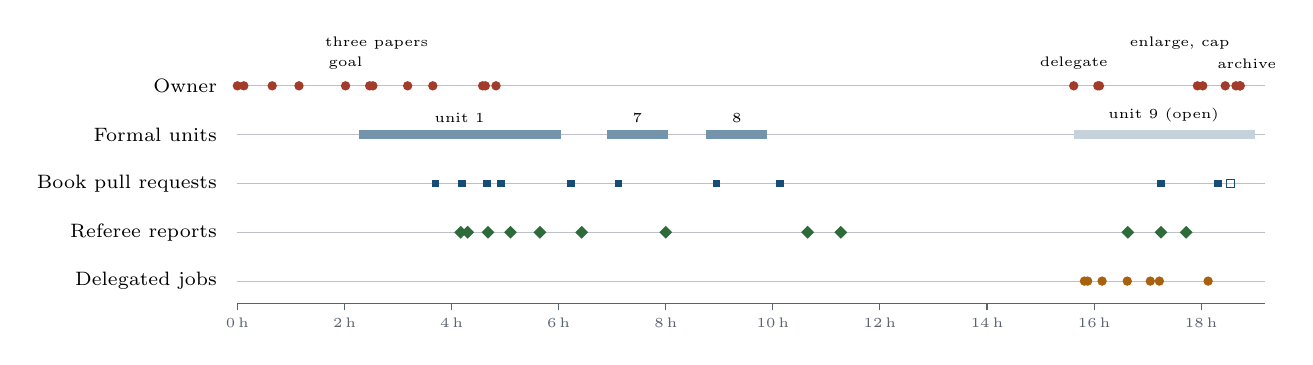
\begin{tikzpicture}[x=0.68cm,y=0.62cm,
  lane/.style={font=\scriptsize,anchor=east},
  ev/.style={circle,fill=humanred,inner sep=1.2pt},
  bk/.style={rectangle,fill=linkblue,inner sep=1.4pt},
  rf/.style={diamond,fill=reviewgreen,inner sep=1.2pt},
  dj/.style={circle,fill=standorange,inner sep=1.2pt}]
\foreach \y/\t in {0/Owner,-1/Formal units,-2/Book pull requests,-3/Referee reports,-4/Delegated jobs}{
  \node[lane] at (-0.2,\y) {\t};
  \draw[planegray!40] (0,\y) -- (19.2,\y);}
\foreach \x in {0,2,...,18}{\draw[planegray] (\x,-4.6) -- (\x,-4.45) node[below=2pt,font=\tiny] {\x\,h};}
\draw[planegray] (0,-4.45) -- (19.2,-4.45);
% owner messages
\foreach \x in {0,0.12,0.65,1.15,2.02,2.47,2.53,3.18,3.65,4.58,4.63,4.83,15.62,16.07,16.10,17.93,18.03,18.45,18.65,18.72,18.73}{\node[ev] at (\x,0) {};}
\node[font=\tiny,above] at (2.02,0.15) {goal};
\node[font=\tiny,above] at (2.6,0.55) {three papers};
\node[font=\tiny,above] at (15.62,0.15) {delegate};
\node[font=\tiny,above] at (17.6,0.55) {enlarge, cap};
\node[font=\tiny,above] at (18.85,0.15) {archive};
% formal units
\draw[line width=3pt,linkblue!60] (2.27,-1) -- (6.04,-1);
\draw[line width=3pt,linkblue!60] (6.90,-1) -- (8.05,-1);
\draw[line width=3pt,linkblue!60] (8.76,-1) -- (9.90,-1);
\draw[line width=3pt,linkblue!25] (15.63,-1) -- (19.0,-1);
\node[font=\tiny,above] at (4.15,-0.95) {unit 1};
\node[font=\tiny,above] at (7.47,-0.95) {7};
\node[font=\tiny,above] at (9.33,-0.95) {8};
\node[font=\tiny,above] at (17.3,-0.95) {unit 9 (open)};
% book PRs merged
\foreach \x in {3.70,4.20,4.66,4.92,6.23,7.12,8.95,10.13,17.25,18.31}{\node[bk] at (\x,-2) {};}
\node[draw=linkblue,inner sep=1.4pt] at (18.55,-2) {};
% referee reports
\foreach \x in {4.17,4.68,8.00,10.65,16.63,4.30,5.10,5.65,6.43,17.25,11.27,17.72}{\node[rf] at (\x,-3) {};}
% delegated jobs (results)
\foreach \x in {15.82,15.88,16.15,16.62,17.05,17.22,18.13}{\node[dj] at (\x,-4) {};}
\end{tikzpicture}
\caption{The first nineteen hours of the AXIOM-$\Omega$ line, in hours after
the owner's first message. Owner messages (red); formal units from
preregistration to merge (bars; unit~9 still open); book pull requests at
merge (filled squares) and the archive pull request at opening (open square);
referee reports (green); results of delegated and adversarial jobs (orange).}
\label{fig:timeline}
\end{figure}

\paragraph{From intent to goal file.} The owner asked how far the material was from a
paper and then asked for a draft that unifies and fills the gaps. When the
first answers listed what could not be derived, the owner corrected the
course: open a goal and keep looping on it. The orchestrator wrote the goal
file of Box~\ref{box:goal}, started a remote formalization agent, and began
running the loop. Half an hour later the owner widened the intent into three
papers and asked that concrete tasks go to subagents.

\paragraph{Rounds, referees and units.} The research loop ran about one round
an hour: by the nineteenth hour the mathematical draft was at round~23 and
the physical draft at round~24, after twelve referee reports. The
formalization line merged three units on the first evening and opened a
fourth the next morning; ten book pull requests carried the stabilized
results back to the book. Table~\ref{tab:caught} lists what the gates caught
along the way.

\begin{table}[htbp]
\centering\scriptsize
\caption{Gate efficacy on the case study: what each gate caught, the kind of
gate, and the outcome.}
\label{tab:caught}
\begin{tabularx}{\linewidth}{@{}>{\raggedright\arraybackslash}p{0.2\linewidth}>{\raggedright\arraybackslash}p{0.17\linewidth}>{\raggedright\arraybackslash}X>{\raggedright\arraybackslash}p{0.2\linewidth}@{}}
\toprule
Gate & Kind & Caught & Outcome \\
\midrule
Library-first search & Machine-assisted search & The first unit's dimension statement was already a frozen theorem & Reused, not re-proved \\
Referee, literature & Fresh context, same family & A ``new'' rigidity theorem was an elementary corollary of Hurwitz's theorem & Cited, not claimed \\
Referee, status & Fresh context, same family & Inputs presented as outputs & Relabelled as hypotheses \\
Referee, counterexample & Fresh context, same family & A claim false as stated & Withdrawn; kept as a refutation \\
Referee, novelty & Fresh context, same family & A ``prediction'' that is a standard ratio & Removed \\
Cross-paper referee, consistency & Fresh context, both papers & Abstracts stronger than their theorems; a cross-citation missing premises & Aligned \\
Referee, physics & Fresh context, same family & Under two of its hypotheses the electroweak sector has no scalar particle & Stated in the draft \\
Adversarial review & Second family, fresh context & Two small gaps in the delegated roundness proof & Repaired; then verified by the first family \\
Cross-paper referee & Fresh context, both papers & The one-sided counterexample leaves a twice-differentiable variant open & Re-derived; variant listed as open \\
Book write-back & Book review & A later result contradicted a sentence of an earlier book update & Corrected \\
Required check & Machine & A missing build cache failed a unit's check & Rule: wait for the cache run, rerun once \\
Owner & Human & Drafts too conservative; too many parallel jobs & Enlarged; capped \\
\bottomrule
\end{tabularx}
\end{table}

\paragraph{Delegation, scale, archive and genre.} On the second morning the
owner allowed hard problems to be delegated. The first job proved a
roundness theorem for the mathematical draft---under continuity and
two-sided invariance the space is compact and isometric to a round sphere of
dimension 1, 3 or 7; a second job reviewed it in a fresh context; the
author-agent verified and wrote it in; a referee confirmed it as stated. It is
a refereed draft result, not yet formalized. Within the next three hours the
owner judged the drafts too conservative and had them enlarged to absorb the
book, capped the parallel jobs when the machine came under memory pressure,
moved the drafts into a \code{paper/} directory of the book repository as an
archive reviewed by a co-author, fixed the genre of this paper, and named the
execution plane as central to the loop.

\paragraph{Observations.} We observe three regularities on the case study.
First, the human inputs were few and short (Section~\ref{sec:steering}), and
each changed the direction of the whole loop within one tick. Second, every
result left the loop with an explicit status: merged Lean module, refereed
draft, open question, hypothesis or programme. Third, every kind of gate
caught something (Table~\ref{tab:caught}): fresh-context referees caught
literature, status and consistency errors in drafts of their own model
family, the other family's adversarial review caught gaps in delegated
proofs, the machine gates caught an infrastructure failure, and the human
caught two matters of scale.

\section{Design principles}
\label{sec:lessons}
Table~\ref{tab:principles} states the design principles of the method, each
with its rationale and the mechanism that implements it.

\begin{table}[htbp]
\centering\scriptsize
\caption{Design principles, their rationale, and the implementing mechanism.}
\label{tab:principles}
\begin{tabularx}{\linewidth}{@{}>{\raggedright\arraybackslash}p{0.3\linewidth}>{\raggedright\arraybackslash}X>{\raggedright\arraybackslash}p{0.19\linewidth}@{}}
\toprule
Principle & Rationale & Implemented in \\
\midrule
1. Let a kernel decide truth; give everything else a status & A draft result is usable at its stated strength & Ledger, status legend, book badges \\
2. Preregister before proving & Naming the expected new content keeps formalization aimed at new mathematics & Preregistration issues \\
3. Search the library before proving & Reuse is cheaper than re-proof and keeps the library dense & Admission rules \\
4. Keep units small, with a stopping rule & A unit ends at merge or at a named obstacle, so progress is always recorded & Goal file, status file \\
5. Refutations and blocked units are results & A closed route tells the next reader where not to go & Status \textsc{refuted}; obstacles in status files \\
6. The author of a draft is never its only reviewer & A fresh reader finds what the author no longer sees & Referee seats, review loop, Mathesis auditor \\
7. Review a numbered snapshot & Every finding points at exact text while authors keep working & Snapshots \\
8. Verify delegated work with a different family & Errors one family makes systematically are caught by the other & Delegation protocol \\
9. The oracle proposes routes; an executing seat verifies them & Ideas come cheaply; verification needs a seat that can run code & Seats \\
10. Put the intent in a file every actor reads & A one-sentence correction takes effect in the next tick & Goal file, queue, memory note \\
11. Externalize state and re-measure after context loss & A line outlives any single context & Queue, memory note, status file \\
12. Delegate routine decisions explicitly; reserve the rest & Routine work runs continuously; authorship and sensitive letters stay with people & Standing grants, routing \\
13. Send only reviewed, exact versions & What was reviewed is what is sent; an uncertain send is looked up & Outreach coordinator \\
14. Close the loop to the problem's authors & The people who posed a problem are its best readers & Outreach \\
15. Broker every credential & One revocation point and narrow reach for each seat & NyxID, CMA \\
16. Scope ownership of shared objects; turn failures into rules & A session stops only processes it started, by recorded identifier, because name or pattern matches reach other sessions' work; each recorded error becomes such a rule & Rules file, goal files \\
\bottomrule
\end{tabularx}
\end{table}

\section{Evaluation methodology}
\label{sec:evaluate}
We propose to evaluate the method by its yield on a fixed cohort of intents:
take the intents stated in a fixed window, follow each for a fixed period, and
record whether it ends in a merged formal unit, a refereed draft, a
refutation, a letter that received an answer, or nothing; record the human
input in messages and the agents' work in jobs and agent-hours; and compare
the findings of fresh-context and cross-family review with those of external
referees on the same snapshots. The fourteen earlier preprints of
Appendix~\ref{app:outputs} form a fixed corpus for a planned comparison of
Mathesis review with an external automated reviewer
(Appendix~\ref{app:study}).

\section{Implications and outlook}
\label{sec:outlook}
\paragraph{What generalises beyond mathematics.} The control channel, the
externalised state, the separation of seats, machines and credentials, the
status vocabulary, review of numbered snapshots by seats other than the
author, cross-family verification of delegated work, and the dissemination
loop to domain experts do not depend on the subject. What is special to
mathematics is the strength of its strongest gate: a proof kernel decides a
formal proposition, and a library of kernel-checked results lets later work
reuse earlier work without re-review. Other sciences need other arbiters in
that position. Candidates are preregistered statistical tests with fixed
analysis plans \citep{nosek}, replication by an independent pipeline,
simulation with conserved-quantity and convergence checks, and closed-loop
laboratory automation with controls, as in robot scientists \citep{king}.
Each is weaker than a kernel, so the status vocabulary must distinguish
evidence levels more finely, and more claims remain at the level of reviewed
draft.

\paragraph{Limits and risks.} We name five risks of the paradigm and the
mechanism of this method that addresses each.
\emph{Error cascades between agents}: an unchecked statement can become the
premise of many later ones. The method attaches a status to every statement,
raises it only through a gate, and keeps refutations as results; the ledger's
retraction rule makes the cost of a correction proportional to its dependent
subgraph.
\emph{Homogeneity of model families}: agents of one family share blind spots,
and language models favour their own generations as evaluators
\citep{panickssery,huang}. The method verifies delegated work across families,
but its referees share the orchestrator's family; making cross-family
refereeing the default is an open design question.
\emph{Provenance and credit}: when agents produce most of the text, the
record of who contributed what becomes the basis of credit. Provenance headers
on every pull request and the records of Table~\ref{tab:records} address the
technical side; authorship conventions for such work remain open.
\emph{Reviewer capacity}: automated production multiplies the material that
experts are asked to read. Fresh-context referees, the Mathesis audit and the
review loop filter what reaches people, and letters go only to the authors of
the problem a result concerns; external review remains the scarce resource.
\emph{Dependence on proprietary models}: the agents run on commercial models.
The proof kernel and the library do not depend on them, and the broker makes
each model route replaceable; the reproducibility of the drafts themselves
remains tied to model versions.

\paragraph{A research agenda.} The paradigm raises measurable questions.
(1) \emph{Human input per verified result}: on the case study, about seven
messages per merged formal unit; how does this ratio scale with the size and
difficulty of a line? (2) \emph{Gate efficacy}: what fraction of errors does
each gate catch, and at what cost, measured on a fixed cohort with external
review as reference? (3) \emph{Cross-family verification}: does verification
by another model family catch errors that fresh-context review by the same
family misses? (4) \emph{Scaling of the ledger}: how do admission rules and
review hold up as the library grows from tens to hundreds of thousands of
modules? (5) \emph{Community review}: how should results produced at machine
rate be routed to human experts without exhausting them? Five design changes
follow from the case study: machine-readable preregistration checked by the
required check; a referee of the other family for every delegated result and
a second reading seat for reviewer edits to letters; long agents designed
for small contexts from the start; explicit budgets for remote agents and
parallel jobs in the goal file; and external referees for the research
drafts.

\section{Limitations}
\label{sec:limits}
The evidence comes from one team. Activity counts measure work done; the
yield of the loop on a fixed cohort of intents has not been measured. Review
is internal so far: referee seats are agents of the orchestrating session,
and the research drafts of the case study have not been reviewed outside
the team; the physics draft's kinematic part reproduces standard quantum
mechanics, and its field part is stated as hypotheses. Several rules,
including preregistration and the judgement of proof shape, are conventions
checked by review. The formal side trails the drafts: the statements of the
Mathesis catalog and most of the research drafts await Lean targets. The
execution plane is operated by the same organization that operates the
research system.

\section{Related work}
\label{sec:related}
\paragraph{Human-in-the-loop systems and automated science.} Supervisory
control, in which a human sets goals and monitors an automated process that
executes them, goes back to work on teleoperation by Sheridan and Verplank,
who also proposed a scale of levels of automation \citep{sheridan};
Parasuraman, Sheridan and Wickens extended it to types and levels of
automation for information acquisition, analysis, decision and action
\citep{parasuraman}. Horvitz formulated principles for mixed-initiative
interfaces, in which initiative passes between person and machine
\citep{horvitz}, and Amershi et al.\ surveyed the role of humans in
interactive machine learning \citep{amershi}. On automated science, King et
al.\ demonstrated a robot scientist that formed and tested hypotheses in a
closed loop \citep{king}; Gil et al.\ argued for amplifying scientific
discovery with AI \citep{gil}; Kitano proposed the Nobel Turing Challenge as a goal
for AI-driven discovery \citep{kitano}; and Wang et al.\ reviewed scientific discovery in the age of
AI \citep{wangsci}. Our method takes the supervisory-control view: the human
controls through a recorded channel, and the machine executes under gates.

\paragraph{AI research systems.} ScientistTwo lets review and rebuttal produce
additional experiments \citep{scientisttwo}; its held-out Stanford threshold
rate changes from 49.0\% to 73.5\% to 69.4\% over rounds zero to two.
Co-Scientist combines hypothesis development with expert-guided validation
\citep{coscientist}; the AI Scientist and its successor study autonomous
manuscript production \citep{aiscientist,scientistv2}; Agent Laboratory uses
agents as research assistants \citep{agentlab}; and Kosmos is an AI
scientist for autonomous discovery \citep{kosmos}. Symposium keeps durable
records of scientific argument \citep{symposium}, VerifiedLab couples
literature work to discovery \citep[Figure 2]{verifiedlab}, and OpenAI4S
organizes persistent execution through sessions and artifact histories
\citep{openai4s}. Our loop adds a proof kernel as the arbiter of formal
claims, a single status vocabulary for everything else, and expert
correspondence as a standing return path.

\paragraph{AI in mathematics and formal proving.} Davies et al.\ show machine
learning guiding mathematicians' intuition \citep{davies}; FunSearch and
AlphaEvolve let evaluators guide program search \citep{funsearch,alphaevolve},
and Georgiev, G\'omez-Serrano, Tao and Wagner report mathematical
exploration and discovery at scale \citep{georgiev}. Several systems
put a proof kernel inside a learning or search loop: Draft, Sketch, and Prove
turns informal proofs into formal sketches \citep{dsp}; LeanDojo and Lean
Copilot connect language models to Lean \citep{leandojo,leancopilot};
LeanAgent studies lifelong learning across repositories \citep{leanagent};
DeepSeek-Prover-V2, Goedel-Prover, Kimina-Prover and Seed-Prover train
large provers for Lean \citep{deepseekprover2,goedel,kimina,seedprover};
AlphaGeometry solves olympiad geometry \citep{alphageometry}; and AlphaProof
and Aristotle reach olympiad-level formal reasoning
\citep{alphaproof,aristotle}. These systems improve the prover; our method
uses provers as seats and supplies the surrounding practice. Collaborative
mathematics at scale has precedents in the Polymath projects
\citep{polymath} and, with Lean as the arbiter, in the Equational Theories
Project \citep{etp}; both coordinate many human contributors, and our loop
coordinates a small team with many agent seats. Our ledger builds on Lean~4
and Mathlib \citep{lean4,mathlib}.

\paragraph{Agents, review and memory.} Software agents such as SWE-agent and
OpenHands give language models a working environment
\citep{sweagent,openhands}; MemGPT manages context beyond a single window
\citep{memgpt}, the problem our queue, memory note and status files address.
Language models do not reliably correct their own reasoning without external
feedback \citep{huang} and favor their own generations as evaluators
\citep{panickssery}; multi-agent debate improves factuality
\citep{du}. These findings motivate our separation of author and referee
seats, fresh contexts, and cross-family review. Preregistration follows the
practice of the empirical sciences \citep{nosek}; PROV and FAIR provide
vocabulary for provenance and reuse \citep{prov,fair}; Thakkar et al.\ study
model feedback on human reviews \citep{thakkar}.

\begin{table}[htbp]
\centering\scriptsize
\caption{Positioning against representative systems (\checkmark\ present;
--- absent or not reported).}
\label{tab:position}
\begin{tabularx}{\linewidth}{@{}>{\raggedright\arraybackslash}p{0.2\linewidth}>{\raggedright\arraybackslash}X cccc@{}}
\toprule
System & Human control channel & Formal arbiter & Cross-model review & Publication & Expert return path \\
\midrule
ScientistTwo \citep{scientisttwo} & Task specification & --- & --- & \checkmark & --- \\
Co-Scientist \citep{coscientist} & Expert guidance and validation & --- & --- & --- & \checkmark \\
AI Scientist \citep{aiscientist} & Task specification & --- & --- & \checkmark & --- \\
AlphaProof \citep{alphaproof} & Problem statement & \checkmark & --- & --- & --- \\
Equational Theories Project \citep{etp} & Human coordination of contributors & \checkmark & --- & \checkmark & --- \\
This method & Intent, correction, standing delegation, limits & \checkmark & \checkmark & \checkmark & \checkmark \\
\bottomrule
\end{tabularx}
\end{table}

\section{Conclusion}
We have presented a human-in-the-loop methodology for automated mathematical
research, modelled as a supervised control system: the human specifies intent
and exercises supervisory control through a recorded channel; actors with
separated seats, machines and credentials derive, check, formalize, publish
and correspond; and gates---check scripts, fresh-context and cross-family
review, and a proof kernel with a single required check---decide which
statements enter the record and with what status. The case study shows a few
short human inputs directing two days of gated work. We have argued that this
division of labour, in which people specify intent, design gates and audit
evidence while machines produce derivations, is a plausible organisation of
research wherever automated derivation is cheap and verification is costly,
and we have stated the questions that would test that argument.

\appendix
\section{Templates}
\label{app:templates}
The templates below are taken from the AXIOM-$\Omega$ line, with local paths,
host names and identifiers replaced by placeholders in angle brackets.

\subsection*{A.1 Goal file (abridged)}
\begin{small}
\begin{verbatim}
# GOAL - <line title>: formalise in the library and write back
You are the formalisation owner for one research line in <library repo>.
Work on <build machine>, in the clone <checkout>.
## 0. Authority and house rules
- The rules file and the skills <...> govern; where this GOAL disagrees,
  they win; record the disagreement in STATUS and continue.
- Preregister before any Lean probe. Name the proposed non-binding facts.
- Edits only in a linked worktree (make worktree). No extra clones.
- Delivery: push, PR, required checks green, MERGED, first dev push
  verified. Merge your own PR when checks are green.
- After each unit: return the worktree; delete files this line created
  outside the repository; report disk usage before and after.
- Shared machine: touch only objects this line created; stop only PIDs
  you started and recorded; never match processes by name or pattern.
- Targeted Lean builds; at most 6 build threads while the load is high.
- Never report a check, proof or coverage that did not happen. A unit that
  does not close is reported with its named obstacle; that is a result.
## 1. Identity and files   (orchestrator session, lane suffix, scratch dir,
   source draft, check scripts, STATUS.md)
## 2. Mathematical content (hypotheses H1-H5; claims C0-C6, each with a
   route; literature to cite, not formalise; proposed non-binding facts;
   Unit 1 fully specified; later units listed)
## 3. Deliverables per unit (Lean + Blueprint, frozen by the canonical
   writer, one PR per unit, preregistration issue linked and settled)
## 4. Round discipline (one round = one unit to MERGED or a named obstacle)
## 5. STATUS file (overwrite after every material step; schema below)
\end{verbatim}
\end{small}

\subsection*{A.2 Tick prompt (translated from Chinese)}
\begin{small}
Advance the line by one round: (1) read the remote agent's state and its
status file on the build machine; if it is idle or blocked, read its log,
give the mathematical solution or the next unit's instruction, and send it to
the agent; when its pull request is green and meets the rules, confirm the
merge and verify the first push on the development branch. (2) Continue the
open derivations in the local draft; write newly derived and numerically
checked results into the draft and recompile; add the relevant literature.
(3) After each delivered unit, clean up: on the build machine delete only the
worktrees this line registered and its temporary files; locally delete build
intermediates. Stop the loop and summarize when all units are delivered and
the draft agrees with the formalization. Touch only this session's objects;
stop processes by recorded identifier, never by name.
\end{small}

\subsection*{A.3 Delegation task file (abridged)}
\begin{small}
\begin{verbatim}
# Task (mathematics; write everything in this directory only)
Context: <paper>/main.tex (read-only). Read its Definition <...>,
Theorem <...>, Section <...>, and open question <...>.
Problem. <exact statement with all hypotheses; what is NOT assumed>
Deliver in RESULT.md: (A) a complete proof (state every hypothesis used;
cite precisely any theorem used), or (B) a counterexample with full
verification, or (C) the strongest partial result you can PROVE, with
the exact remaining gap and the natural extra hypothesis that closes it.
Provide check.py (numpy only) for every identity or example, and run it.
Mark what is proved, what is cited (and whether you verified it), and
what is conjecture. Do not overclaim.
Status table: PROVED / LEAN (file::name) / CLASSICAL (exact reference) /
HYPOTHESIS / CONJECTURE / PROGRAMME / REFUTED (counterexample and
corrected statement); list "what a referee should attack first".
\end{verbatim}
\end{small}

\subsection*{A.4 Adversarial-review prompt (abridged)}
\begin{small}
\begin{verbatim}
# Task: adversarial verification of a claimed proof
../<job>/RESULT.md claims to prove: <statement>.
You are a hostile referee. Find errors. Go through RESULT.md sentence by
sentence and for EVERY inference decide: correct / gap (state exactly what
is missing; repair it if you can) / wrong (counterexample or failing step).
Check the exact hypotheses of every cited theorem. Look for hidden
hypotheses. Try to construct counterexamples to the theorem itself and say
which hypothesis kills each. Write REVIEW.md: verdict (correct / correct
after listed repairs / wrong), numbered findings with severity, complete
repairs, and a corrected statement with minimal hypotheses. Add a check
script for anything testable. Be exact; do not be polite.
\end{verbatim}
\end{small}

\subsection*{A.5 Referee prompt (abridged)}
\begin{small}
\begin{verbatim}
You are an independent, hostile-but-fair referee. Find every error, gap
and overstatement, and say which results you could verify.
Manuscript (read-only numbered snapshot): <snapshot>/main.tex.
The authors' check script: <snapshot>/check.py. Their gap list: read it
LAST, after forming your own view, so that it does not anchor you.
Write ONLY inside <referee folder>/ (report.md and any scripts).
For EVERY theorem, lemma, proposition and corollary: restate the claim;
check the proof line by line; test it on examples and near-counterexamples
of your own (exact arithmetic where it matters); check that every
hypothesis is used and every used hypothesis is stated; check boundary
cases. Priority targets: <the new core results>.
Report: blocking findings and minor findings, each with the statement it
concerns; what you verified; novelty and literature.
\end{verbatim}
\end{small}

\subsection*{A.6 Status file (example)}
\begin{small}
\begin{verbatim}
updated: <UTC time>
codex_session: <id>
unit: 9
phase: pr-open        # prereg|probe|implement|review|pr-open|merged|cleaned|blocked
issue: <issue url>
pr: <pull request url>
worktree: <path>
branch: <lane>/<topic>-<suffix>
build_pids: -
frozen: -
obstacle: required check failed: build cache missing for this commit
next: wait for the cache-producing run of this commit, then rerun once
\end{verbatim}
\end{small}

\subsection*{A.7 Preregistration issue and pull-request header}
A public preregistration issue (for example trureturing issue~31739
\citep{prereg31739}) carries: the hypotheses and the exact statement; the
proposed new facts and the frozen declarations to be reused; the admission
basis; the state of the escape audit; the creating sessions with their resume
commands; and, at settlement, the merged pull request, the commit, the
required-check run and the verification of the first push. A pull-request
header begins:
\begin{small}
\begin{verbatim}
Codex session: <id> (`codex resume <id>`). Orchestrator: <id>
(`claude --resume <id>`). Skills: <skills used>.
<what the unit proves; what is new; what is reused>
Validation: <targeted compilation; report; axioms used>
Declaration judgment: proof_shape and admission_basis per declaration,
with the consumer of every bind-only helper.
New frozen identifiers and state-file digests.
Preregistration and settlement: <issue>.
\end{verbatim}
\end{small}

\subsection*{A.8 The rules file in brief}
\begin{enumerate}[leftmargin=*,itemsep=0pt]\small
\item Only declarations checked by the Lean kernel, with their proof terms and axiom closure, carry truth; everything else is input or bookkeeping.
\item Every statement has a status; what cannot be decided is marked \code{open}.
\item Correctness is decided by machines and by independent review seats; people authorize irreversible actions and choose direction.
\item Preregister the expected new content in a public issue before probing; a different witness needs a new preregistration.
\item Search the library, Mathlib and admissible libraries before proving; import exact hits.
\item Add no bind-only declaration, except a helper with a live consumer or the conclusion of a preregistered open-problem settlement.
\item A first freeze needs an escape witness or the settlement of a named open problem.
\item Bounded enumerations and certified instances enter only as typed refutations of a named claim.
\item Register each new public theorem's escape against a readout template; registration verdicts are warnings.
\item Formalization does not change the judges; a blocking judge is reported in an issue.
\item One required check; candidate code is executed and the base is read as data; strict up-to-date merging is off by ruling.
\item Work in a linked worktree; checkpoint after every recoverable step; verify the first push after a merge.
\item Every pull request and issue discloses the skill, the seats, their model families and the creating session.
\item Statements about the system cite a reading; vague wording does not replace a measurement.
\item Processes are stopped only by the session that started them, by recorded identifier.
\item A new kind of error gets a written handling and, where possible, a machine check.
\end{enumerate}

\subsection*{A.9 Outreach kit in generic form}
\paragraph{Hold codes.} Wrong mathematics; trivial; straw man; wrong domain;
already settled; unverifiable central claim; literature unavailable; no
current confirmed author; unresolved identity; declined; active reply
thread; duplicate or uncertain send; owner decision needed; stale policy;
Lean result not on the development branch or with gaps; no genuinely open
question; invalid note.

\paragraph{Review rubric.} Confirm the item, version and hashes of the exact
packet; read the posed statement in its source and check that it is still
open in the latest preprint, journal version and later literature; check the
central mathematics independently with a small calculation; check every
recipient against the paper, the refusal table and thread ownership; return
PASS, BOUNCE (with concrete feedback) or HOLD (with a code).

\paragraph{Records.} A verdict records the task, its revision, the result
hash, the workflow hash, the reviewer, the verdict, the reason and the
evidence reference, and is HMAC-authenticated. A decision envelope records
the task, the result hash, the owner's answers by question, the evidence
reference and the reviewer.

\section{Repositories and versions}
\label{app:repro}
The figures in this paper are as of 20 November 2026.

\begin{table}[htbp]
\centering\small
\caption{Repositories and versions behind the figures in this paper.}
\label{tab:repro}
\begin{tabularx}{\linewidth}{@{}>{\raggedright\arraybackslash}p{0.3\linewidth}>{\raggedright\arraybackslash}X@{}}
\toprule
Source & Version and figures \\
\midrule
trureturing \citep{trureturingrepo} & Branch \code{dev} at \code{d3cafbe}: 16{,}436 Lean files, 14{,}832 frozen modules, 5 skills; formalization units in pull requests 31765, 31864 and 31928, preregistered in issues 31739, 31839 and 31913 \\
trureturing-books \citep{booksrepo} & Book pull requests 564, 566, 568, 569, 570, 575, 593, 602, 625 and 628; archive pull request 630 \\
Mathesis \citep{mathesisrepo} & Branch \code{develop} at \code{e544a7b}; referee prompts in \code{api/crates/layer3-review/src/referee_prompts.rs} \\
Mathesis catalog \citep{catalogrepo} & Commit \code{3f4c6e9}: 54 papers, 47 with DOI, 352 statements \\
Outreach control repository (private) & Aggregate counts from its contact, result, note and submission tables \\
NyxID \citep{nyxid}, CMA \citep{cma}, heca \citep{heca} & NyxID command-line client 0.7.1 and public documentation; CMA public README; heca 0.1.0-nightly-20260905-1 \\
\bottomrule
\end{tabularx}
\end{table}

\section{Earlier outputs}
\label{app:outputs}
Before the present loop, the same team produced public coauthored papers. On
10 November 2026 we checked forty candidate identities against primary arXiv
records and retained fourteen distinct preprints that list both Haobo Ma and
Wenlin Zhang; thirteen list further coauthors. The inventory is
identity-checked; the proofs and experiments were not rerun, and the
summaries below report what the preprints state. Exact versions are in
Appendix~\ref{app:inventory}.

The entanglement-of-formation preprint states a proof of coincidence of the
discrete and continuous definitions on the whole state space, allowing
infinite values \citep{eof}; the Gaussian preprint reports, for centered
one-mode continuous-variable Gaussian states, positivity of a signed Wigner
periodization in every odd dimension $d\geq3$ under the one-mode uncertainty
condition \citep{gaussian}; the generalized-fidelity preprint states failure
of the data-processing inequality for the induced generalized
Bures--Wasserstein distance in every dimension $n\geq2$ \citep{fidelity}. The
generalized Petersen graph preprint reports
\begin{equation}
 Z(P(n,3))=8\quad(n\geq13),\qquad Z(P(n,4))=10\quad(n\geq18),
\end{equation}
with sharp thresholds, a Lean formalization of the $k=3$ stabilization theorem
and separately checked DRAT certificates for the $k=4$ case \citep{petersen}.
For fixed nonempty source words, the block-exchange insertion preprint states
that after a block exchange from a minimum mask of degree $r$, the minimum
insertion degree over masks with commuting source projections is exactly
$r-1$, while general block-exchange descent and Singleton No-Gap remain open
\citep{insertion}. Under uniform transmission, the entropy preprint identifies
exactly the two alternating received words as maximizers for binary
two-deletion channels at every positive received length; for two insertions
the same characterization holds from received length five, and its
three-error maximizers are certified only over finite ranges
\citep{entropy}. Further outputs concern sub-quorum colorings, well-covered
graph powers, residue sums, a nested recurrence, cellular automata over the
Klein four-group and a cyclic two-qutrit family
\citep{subquorum,wellcovered,residues,padovan,cellular,qutrit}. The EQT2
solver returns certificates replayed as Lean terms or checked by a
deterministic judge \citep{eqt2}, and the routing study measures model
selection of proof-mechanism labels over Lean-verified objects
\citep{routing}.

\section{Planned evaluation of mathematical review}
\label{app:study}
We plan to compare Mathesis review with the Stanford Agentic Reviewer on the
fourteen fixed preprints, stratified by subject and evidence type. For each
run we freeze the PDF bytes, visible page range, reviewer version, rubric
version and raw response. The Stanford service reports seven dimensions and
a final score calibrated to ICLR 2025 reviews, with Spearman correlations of
0.41 between human reviewers and 0.42 between its score and a human reviewer
on 147 test submissions \citep{stanford}; applying it to mathematics is a
domain transfer. Domain adjudicators assess each concrete concern against the
mathematics and literature; the outcomes are the fraction of substantive
concerns independently supported, detection of confirmed defects, and
unsupported criticisms.

Mathesis outputs categorical judgments with reasons and witnesses
(Appendix~\ref{app:rubric}). An optional numeric reading uses the finite
information-escape definitions in trureturing \citep{escape}. Fix a finite
set $X$ with $|X|\geq2$, a finite occurrence index set $I$ and readouts
$r_i:X\to Y_i$. For $S\subseteq I$,
\begin{align}
 E(S)&=\{(x,y)\in X^2:x\ne y,\ r_j(x)=r_j(y)\text{ for all }j\in S\},
 \label{eq:pairs}\\
 \varepsilon(S)&=\frac{|E(S)|}{|X|(|X|-1)},\qquad
 \delta_i=\varepsilon(I\setminus\{i\})-\varepsilon(I).
 \label{eq:escape}
\end{align}
Since $E(I)\subseteq E(I\setminus\{i\})$, $\delta_i\geq0$ counts the ordered
pairs distinguished by $r_i$ alone. For $X=\{00,01,10,11\}$ with first-bit and
second-bit readouts, $\varepsilon(I)=0$ and $\delta_i=4/12=1/3$; adding a
duplicate first-bit readout makes the original occurrence's contribution
zero, so a zero marginal value can indicate redundancy. A paper-specific
reading requires an explicit arena, catalog and correspondence to the claim;
readings from different arenas are not compared.

\section{Versioned public output inventory}
\label{app:inventory}
The following fourteen arXiv preprints were identity-checked against primary
arXiv metadata on 10 November 2026. Titles identify the complete works; scopes
summarize their reported contributions.
% Generated by scripts/render_corpus.py; edit the JSON manifest.
\begingroup\small
\setlength{\LTpre}{4pt}\setlength{\LTpost}{4pt}
\begin{longtable}{@{}p{0.23\linewidth}p{0.72\linewidth}@{}}
\caption{Public output inventory, with exact arXiv versions.}\label{tab:corpus}\\
\toprule Version and field & Work and reported scope \\
\midrule\endfirsthead
\toprule Version and field & Work and reported scope (continued) \\
\midrule\endhead
\midrule\multicolumn{2}{r}{\footnotesize Continued on next page}\endfoot
\bottomrule\endlastfoot
\arxiv{2607.04534v1}\par formal algebra and model evaluation & Mechanism-level routing failure in LLMs over Lean-verified algebraic structures \citep{routing}\par\smallskip Proof-mechanism routing over Lean-verified algebraic objects \\[9pt]
\arxiv{2609.00706v1}\par automated reasoning & A Certificate-Producing Cascade for Equational Implication: The SAIR EQT2 Stage 2 Solver \citep{eqt2}\par\smallskip Certificate-producing equational implication solver \\[9pt]
\arxiv{2609.09753v3}\par quantum information & Generalized Fidelity, the Data Processing Inequality, and Convexity \citep{fidelity}\par\smallskip Data-processing and convexity obstructions for generalized fidelity \\[9pt]
\arxiv{2609.25128v4}\par graph theory & Sub-quorum colorings of graphs \citep{subquorum}\par\smallskip Structural bounds, algorithms and exact sub-quorum coloring values \\[9pt]
\arxiv{2609.33421v1}\par sequences and automata & A Padovan-automatic description of a nested recurrence \citep{padovan}\par\smallskip Finite-state description and exact properties of a nested recurrence \\[9pt]
\arxiv{2610.05623v2}\par quantum information & Approximation of a continuous-variable Gaussian state by discrete-variable quantum states \citep{gaussian}\par\smallskip Positivity and trace-norm-controlled discrete Gaussian approximation \\[9pt]
\arxiv{2610.18816v2}\par quantum information & On the coincidence of discrete and continuous definitions of Entanglement of Formation \citep{eof}\par\smallskip Coincidence of discrete and continuous entanglement-of-formation definitions \\[9pt]
\arxiv{2610.20329v1}\par cellular automata & Generation by lazy and invertible cellular automata over the Klein four-group \citep{cellular}\par\smallskip Characterization and cardinalities of a generated cellular-automaton submonoid \\[9pt]
\arxiv{2610.24059v1}\par graph theory & Sharp zero forcing numbers for the generalized Petersen graphs $P(n,3)$ and $P(n,4)$ \citep{petersen}\par\smallskip Sharp zero forcing numbers for two generalized Petersen graph families \\[9pt]
\arxiv{2610.29608v1}\par number theory & Residue Sums Modulo Products of Two Distinct Odd Primes \citep{residues}\par\smallskip Centered residue sums for cyclic subgroups modulo two odd primes \\[9pt]
\arxiv{2610.39941v1}\par combinatorics on words & Block-exchange descent for insertion: commuting projections and minimum masks \citep{insertion}\par\smallskip Block-exchange descent under commuting source projections; bounded computations \\[9pt]
\arxiv{2611.01064v1}\par information theory & Maximal input entropy for binary two-deletion and two-insertion channels \citep{entropy}\par\smallskip Exact entropy-maximizing binary words for two-deletion and two-insertion channels \\[9pt]
\arxiv{2611.03956v1}\par graph theory & Well-Covered Powers: Cartesian Products and Cayley Graphs \citep{wellcovered}\par\smallskip Well-covered graph powers, Cartesian products and Cayley classifications \\[9pt]
\arxiv{2611.04568v1}\par quantum information & Time-invariant negativity and persistent bound entanglement in a cyclic two-qutrit family \citep{qutrit}\par\smallskip Exact entanglement regions and dynamics for a cyclic two-qutrit family \\[9pt]
\end{longtable}
\endgroup


\section{Mathematical review rubric}
\label{app:rubric}
The planned study uses the following distinctions from the Mathesis review
methodology.

\paragraph{Correctness.}
\status{correct}, \status{gap}, \status{error}, or \status{not\_checked}
records the bounded assessment of the source argument, with the claim,
relevant assumptions, checked steps and any unresolved inference. A
categorical judgment is distinct from a kernel-check receipt.

\paragraph{Proof content relative to prerequisites.}
\status{content}, \status{bind\_only}, or \status{undetermined} describes
whether a live deduction contains a construction, computation or estimate
beyond instantiation, assumption substitution, projection, recombination and
normalization of explicit prerequisites. A witness for content must lie on
the proof path supporting the conclusion.

\paragraph{Literature comparison.}
\status{supported}, \status{unsupported}, or \status{insufficient} describes
the evidence for the comparison actually performed, with the relevant prior
statements and how their assumptions and conclusions relate to the submitted
claim.

\paragraph{Utility.}
A category, rationale and evidence status identify the question or use a
result supports. This field has no universal scalar score.

\paragraph{Concern adjudication.}
Each substantive concern receives a precise target statement, the reviewer's
reason and an independent mathematical adjudication. Revision records keep
the original and revised claims and distinguish repair, narrowing,
withdrawal, confirmation and unresolved outcomes. Escape readings, when
available, keep the construction of
Equations~\eqref{eq:pairs}--\eqref{eq:escape}.

\section*{Statement on the use of AI}
This paper was drafted and revised by Claude Opus 5.5 subagents directed by a
coordinating Claude Code session running Claude Fable 5.2, the same session
that orchestrated the case study; referee and reader rounds on the paper
were run by Claude Opus 5.5 subagents of that session. The system it
describes uses Claude, OpenAI Codex and GPT Pro as stated in the text.
Verification of this version by the listed authors is in progress.

\bibliographystyle{plainnat}
\bibliography{references,corpus}
\end{document}

